\documentclass[a4paper, 11pt, oneside]{extbook}\usepackage[T1]{fontenc}
\usepackage[utf8x]{inputenc}
\usepackage[italian]{babel} %Lingua italiana per gli standard e gli accenti
\usepackage{geometry}
\usepackage{courier}
\usepackage{pdfpages}
\usepackage{amssymb}
\usepackage{minted}
\usepackage{float}
\usepackage{tabularx}
%\usepackage{amsthm}
\usepackage{amsmath}
\usepackage{tikz}
\usepackage[bookmarks]{hyperref}
\newgeometry{
	left=   1.5 in,
	bottom= 1.5 in,
	right=  1 in,
	top=    1 in
}

\usepackage{fancyhdr}

% Grafica
\usepackage{graphicx,pstricks}
\usepackage{graphics}
\usepackage{subfigure}

%
%Algorithm
\usepackage{algorithm}
\usepackage[noend]{algpseudocode}

\setlength\headheight{44.2pt}
%Page Style
\usepackage{setspace}
%\setstretch{2.5} 
\doublespace
%
%%\cfoot{\thepage}
%\lhead[]{}
%\rhead[]{\leftmark}

\pagestyle{fancy}{
%	\lhead{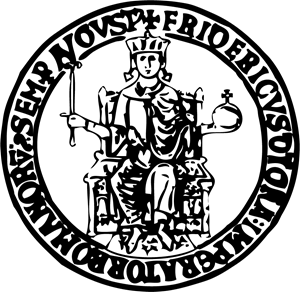
\includegraphics[scale=0.3]{img/logo.png}}
	%	\rhead{\footnotesize{\leftmark}}
	\rhead{\footnotesize{\leftmark}}
	%	\rfoot{\thepage}
}

%\fancyfoot[CE,CO]{\leftmark}
%\fancyfoot[LE,RO]{\thepage}
\renewcommand{\footrulewidth}{1pt}
\linespread{1}

%Other
\usepackage{comment}
\usepackage{amsmath}

%Testo riempitivo
\usepackage{lipsum}




\begin{document}
	\begin{titlepage}
	\begin{center}
		\vspace*{1cm}
		
		\Huge
		\textbf{Università degli Studi di Napoli \\ "Federico II"}
		
		\vspace{0.5cm}
		\LARGE
		Scuola Politecnica e delle Scienze di Base\\
		Corso di Laurea Magistrale in Ingegneria Informatica
		
		\vspace{1.5cm}
		
		\textbf{Giuseppe Francesco Di Cecio - M63001211}
		\\
		\textbf{Nicola D'Ambra - M63001223}
		\\
		\textbf{Emma Melluso - M63001176}
		
		\vspace{2cm}
		
		
		
		\vspace{0.5cm}
		\LARGE
		\textbf{Elaborato di \textit{Impianti di Elaborazione}}
		\vfill
		
		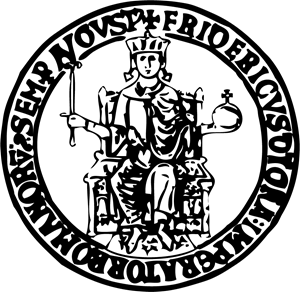
\includegraphics[width=0.2\textwidth]{img/logo.png}
		
		\Large
		Università degli Studi di Napoli \textit{Federico II}\\
		Napoli\\
		A.A 2020/2021
		
	\end{center}
\end{titlepage}

	\frontmatter						%Numerazione romana
	

	{\setstretch{1.5}					%Indice
		\tableofcontents
	}
	
	\backmatter							%Inizio numerazione capitoli
	\mainmatter							%Numerazione pagine
	\chapter{Benchmark}
L'obiettivo dell'esercizio è quello di confrontare due sistemi con lo stesso sistema operativi, ma processori differenti, utilizzando il benchmark \textit{Nbody}. Esso simula l'evoluzione di N corpi celesti, sotto l'influenza della forza di gravità ed è molto utile per confrontare le prestazioni tra i due sistemi, dato che stressa:
\begin{itemize}
	\item \textbf{CPU}
	\item \textbf{Sottosistemi Floating-Point}
	\item \textbf{Chiamate ricorsive}
\end{itemize}
La complessità dell'algoritmo che lo implementa è un \textit{O($n^2$)}.

\section{Sistemi}
Il confronto avviene tramite due macchine virtuali, su architetture diverse. Ogni macchina virtuale però è stata dotata delle stesse caratteristiche e prestazioni, in modo da ridurre il più possibile l'eterogeneità tra i due sistemi fisici. L'unico fattore su cui non si può agire è il processore. 
\\Per rendere il confronto quanto il più possibile affidabile è stata usata anche la stessa versione dell'hypervisor (in questo caso VirtualBox).
\begin{table}[H]
	\begin{center}
		\begin{tabularx}{0.49\textwidth}{|c|X|}
			\hline
			\multicolumn{2}{|c|}{\textbf{Sistema 1}} \\
			\hline
			\textit{CPU} & Intel Core i7-7500U 7th Generation - 2.70 GHz \\
			\hline
			\textit{Memoria Centrale} & 2 GB \\
			\hline
			\textit{Hard-Disk} & 25 GB - SSD \\
			\hline
			\textit{Memoria Video} & 16 MB \\
			\hline
			\textit{OS} & Xubuntu 20.04 LTS - 64bit \\
			\hline
		\end{tabularx}
		\begin{tabularx}{0.49\textwidth}{|c|X|}
			\hline
			\multicolumn{2}{|c|}{\textbf{Sistema 2}} \\
			\hline
			\textit{CPU} & Intel Core i5-5700U 5th Generation - 2.20 GHz\\
			\hline
			\textit{Memoria Centrale} & 2 GB \\
			\hline
			\textit{Hard-Disk} & 25 GB - SSD \\
			\hline
			\textit{Memoria Video} & 16 MB \\
			\hline
			\textit{OS} & Xubuntu 20.04 LTS - 64bit \\
			\hline
		\end{tabularx}
	\end{center}
\end{table}
Ogni macchina virtuale è stata dotata di 2 processori.

\section{Test e Risultati}
Su entrambi i sistemi è stato avviato lo script \textit{launch\_nbody.sh}, con i seguenti parametri di input:
\begin{minted}[framesep = 1mm,
	fontsize = \footnotesize,
	breaklines,
	]{PYTHON}
	./launch_nbody.sh -r 25 -n N
\end{minted}
Esso non fa altro che lanciare l'eseguibile \textit{nbodySim} per un numero di ripetizioni impostato a 25. 
\textit{nbodySim} esegue sul sistema l'algoritmo che implementa il benchmark in questione.
\\
Lo script è stato eseguito facendo variare di volta in volta N:
\begin{equation*}
	N = \begin{bmatrix}
		10 & 100 & 500 & 1.000 & 5.000 & 10.000 & 50.000 & 100.000 & 500.000 & 1.000.000
	\end{bmatrix}
\end{equation*}
L'output fornito da \textit{nbodySim} consiste nel tempo d'esecuzione (in microsecondi) impiegato dal sistema per eseguire l'algoritmo. 
Dunque per ogni valore di N sono state effettuate 25 misurazioni, ciascuna delle quali è stata collezionata in un file \textit{.csv} per poter poi essere processata attraverso il seguente script MATLAB
\begin{minted}[framesep = 1mm,
	fontsize = \footnotesize,
	breaklines,
	]{MATLAB}
%% Read 
N = [10 100 500 1000 5000 10000 50000 100000 500000 1000000];
sys1 = zeros(1, length(N));
sys2 = zeros(1, length(N));
index = 1;

for i=N
	path1 = strcat('Emma/data',num2str(i, '%d'),'.csv');
	path2 = strcat('Peppe/data',num2str(i, '%d'),'.csv');
	samples = readtable(path1);
	samples = table2array(samples(:,2));
	sys1(index) = mean(samples);
	samples = readtable(path2);
	samples = table2array(samples(:,2));
	sys2(index) = mean(samples);
	index = index +1;
end

%% Grafico
figure;
loglog(N,sys1./1000,'LineWidth', 2);
hold on;
loglog(N,sys2./1000,'LineWidth', 2);
grid;
legend('SYS 1', 'SYS 2');
title('Grafico in scala logaritmica');
xlabel('Dimensione dei dati');
ylabel('Tempo di esecuzione [ms]');

figure;
semilogx(N,sys1,'LineWidth', 2);
hold on;
semilogx(N,sys2,'LineWidth', 2);
grid;
legend('SYS 1', 'SYS 2');
title('Grafico in scala normale');
xlabel('Dimensione dei dati');
ylabel('Tempo di esecuzione [ms]');
\end{minted}
Il quale fa una media dei 25 tempi di risposta e ne plotta il grafico, al variare di N, sia in scala normale che in scala logaritmica per evidenziare nel dettaglio le differenze tra i due sistemi.
\begin{figure}[H]
	\centering
	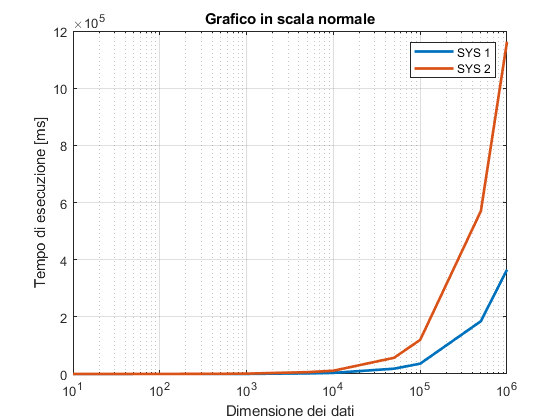
\includegraphics[width=0.8\textwidth]{img/hw0/grafico_naturale.png}
	\caption{\textit{Confronto andamento tempi di risposta sys1 e sys2}}
\end{figure}
\begin{figure}[H]
	\centering
	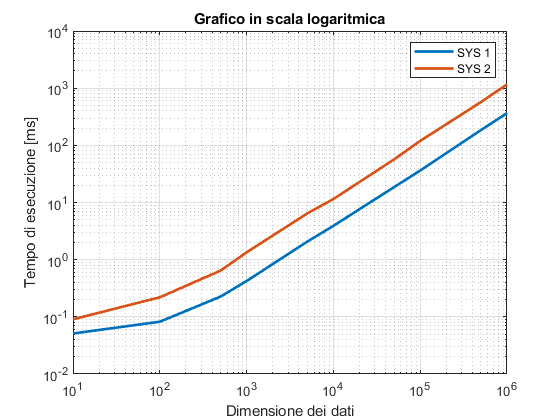
\includegraphics[width=0.8\textwidth]{img/hw0/grafico_log.png}
	\caption{\textit{Confronto andamento tempi di risposta - scala logaritmica}}
\end{figure}
Quindi il primo sistema è con evidenza quello più performante. Le differenze si percepiscono a vista d'occhio già a partire da \textit{N > $10^4$}.
\\Il motivo principale di tale differenza è proprio l'eterogeneità dei processori. Per quanto i due sistemi possano essere simili, il sistema più performante (Sistema 1) è dotato infatti non solo di un processore di architettura più avanzata, ma anche di alcune generazioni successive.
	\chapter{Workload Characterization}
Il dataset di partenza è composto da \textbf{3000 righe} e \textbf{24 colonne}, ciascuna delle quali rappresenta uno dei parametri del sistema oggetto di studio. Si tratta di parametri caratterizzanti l'esecuzione di vari Threads su un sistema operativo.
\\In particolar modo le colonne con prefisso $Vm$ rappresentano informazioni sulla memoria virtuale occupata e utilizzata dai Threads, mentre le altre colonne rappresentano informazioni di carattere generale, come memoria libera, numero di threads, pagine inattive ecc.

\section{Filtraggio}

\subsection{Colonne Identiche}
Innanzitutto osservando il workload e effettuando un grafico delle distribuzioni è possibile rendersi conto della presenza di ben 4 colonne costanti:
\begin{itemize}
	\item \textbf{Active}
	\item \textbf{AnonPages}
	\item \textbf{AvbLatency}
	\item \textbf{Error}
\end{itemize}
Tali colonne in quanto costanti non spiegano varianza, dunque possono essere tranquillamente trascurate ai fini dell'analisi.
\\Osservando le distribuzioni dei parametri \textbf{WriteBack} e \textbf{MemFree} si sono notate alcune caratteristiche comuni. Per avere una maggiore chiarezza si è preferito calcolare la matrice delle correlazioni su questi due parametri.
\begin{figure}[H]
	\centering
	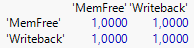
\includegraphics{img/hw1/correlazione_mem_writeback.png}
	\caption{\textit{Matrice di correlazione tra MemFree e WriteBack}}
\end{figure}
Osservando la matrice appare evidente che le due colonne sono esattamente identiche, fornendo quindi la stessa informazione. Per questo motivo si è deciso di trascurare una delle due, in particolare quella di WriteBack.
\\Le 24 colonne iniziali sono state ridotte a 19 colonne, riducendo il dataset di un numero di osservazioni pari a:
\begin{equation}
	n_{dati} = 3.000 \times (24 - 19) = 15.000
\end{equation}

\subsection{Outlier}
Gli outliers sono valori anomali all'interno dell'insieme di osservazioni, in altre parole sono valori che si discostano notevolmente dagli altri valori dell'insieme. 
Essendo valori anomali la loro frequenza di occorrenza è bassa rispetto agli altri valori e ciò li porta ad essere identificati all'esterno del range interquartile. 
In alcuni casi gli outlier possono essere eliminati ma ciò è possibile solo a monte di una analisi accurata. Tali valori infatti influiscono sulle analisi statistiche in modo considerevole e non sempre rappresentano situazioni trascurabili per l'analisi da svolgere .
Osservando attraverso box plot e grafici di distribuzione l'andamento dei seguenti parametri :
\begin{itemize}
	\item \textbf{VmSize} (quanta memoria virtuale utilizza l'intero processo);
	\item \textbf{VmHWM} (di quanta RAM il processo necessita al massimo);
	\item \textbf{VmRSS} (quanta RAM il processo sta correntemente usando);
	\item \textbf{VmPTE} (quanta memoria Kernel è occupata dalle entries della tabella delle pagine);
\end{itemize}
\begin{figure}[H]
	\centering
	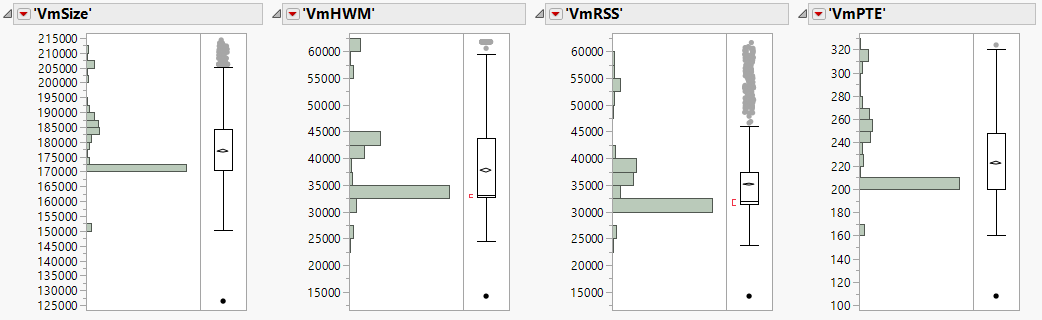
\includegraphics[width=1\textwidth]{img/hw1/outlier_vm.png}
	\caption{\textit{Grafici di distribuzione di VmSize, VmHWM, VmRSS, VmPTE}}
\end{figure}
Si è notato che essi presentano un outlier isolato (in basso ad ogni grafico) in comune associato alla prima riga del dataset. Analizzando gli altri parametri (\textit{MemFree}, \textit{Dirty}, \textit{PageTables}, \textit{Buffer}, ...) è stato possibile evidenziare che anche per la maggior parte di essi lo è, ma non è un punto isolato. 
\\L'ipotesi fatta è che con molta probabilità le prime righe del dataset (da 0 a 100 circa), rappresentano la fase di avvio del processo e l'outlier oggetto di studio è la prima istanza di questa fase. Dato che l'obiettivo della caratterizzazione del workload è quello di analizzare le prestazioni a regime del sistema oggetto di studio (in questo caso), si è deciso di trascurare quel singolo outlier. Tuttavia è bene notare che in ogni caso le informazioni riguardo questa fase di avvio non saranno del tutto perse dato che è stato rimosso un singolo punto e non tutti i punti che la rappresentano.
\\
\vspace{0.5cm}
\\
Un secondo outlier che può essere agevolmente rimosso è la riga 512 in cui il parametro \textbf{Slab} assume valore 4. 
\begin{figure}[H]
	\centering
	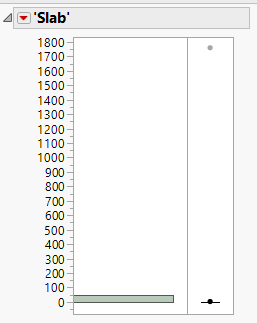
\includegraphics[width=0.4\textwidth]{img/hw1/outlier_slab1.png}
	\caption{\textit{Grafico di distribuzione di Slab}}
\end{figure}
Oltre ad avvicinarsi molto al valore medio assunto da Slab (zero), esso risulta essere un outlier solo per il parametro stesso dato che per gli altri è un valore compreso tra i quartili. Una sua rimozione quindi non influenza gli indici di caratterizzazione sintetica dei parametri del workload complessivo.
\\
\vspace{0.5cm}
\\
Un terzo outlier è il valore 1760 del parametro \textit{Slab}, associato alla riga 90 del workload.
\begin{figure}[H]
	\centering
	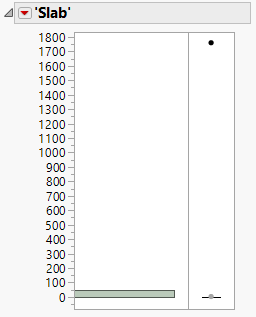
\includegraphics[width=0.4\textwidth]{img/hw1/outlier_slab2.png}
	\caption{\textit{Grafico di distribuzione di Slab}}
\end{figure}
Rispetto al precedente, tale outlier richiede un' analisi più approfondita visto che influenza significativamente l'andamento di parametri quali \textit{Mapped} e \textit{PageTables}. Per descrivere meglio la dipendenza tra questi parametri si può effettuare un grafico tra il numero dell'osservazione e il valore assunto da \textit{Mapped}, analogo discorso con \textit{PageTables}.	
\begin{figure}[H]
	\centering   
	\subfigure{	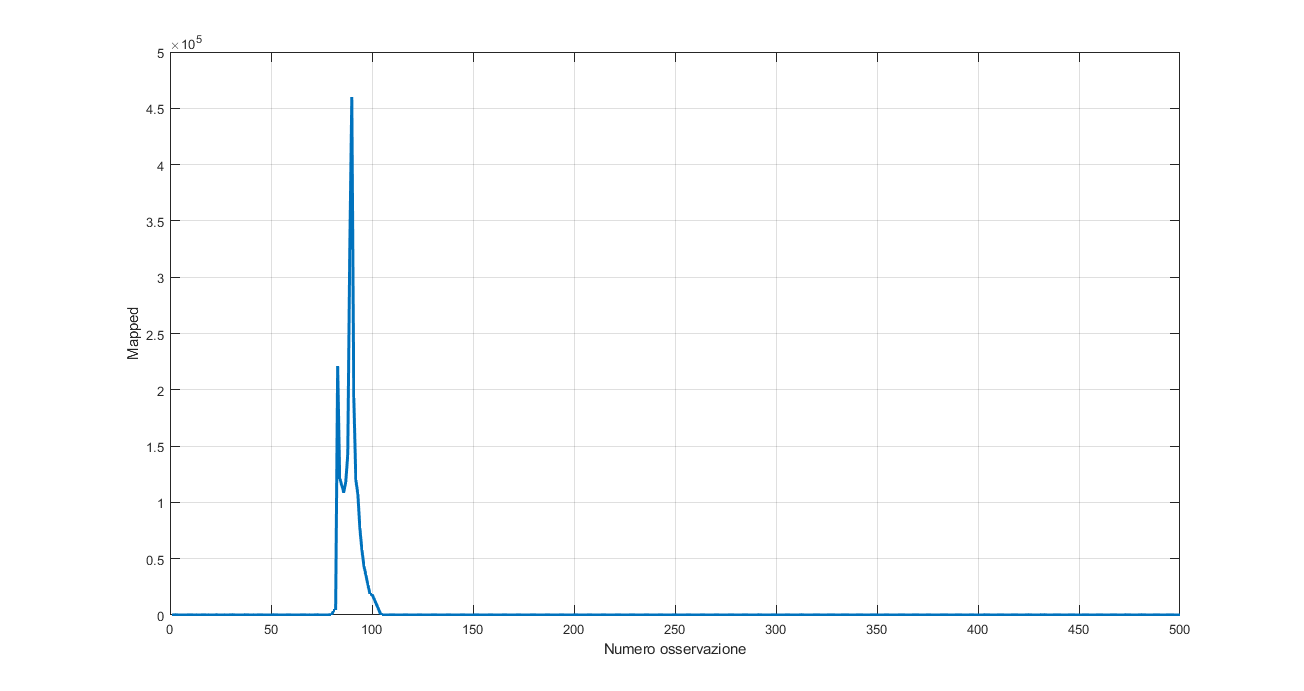
\includegraphics[width=\textwidth]{img/hw1/mapped.png}}
	\caption{\textit{Grafico tra numero di osservazione e valore assunto dal parametro Mapped}}
	\subfigure{	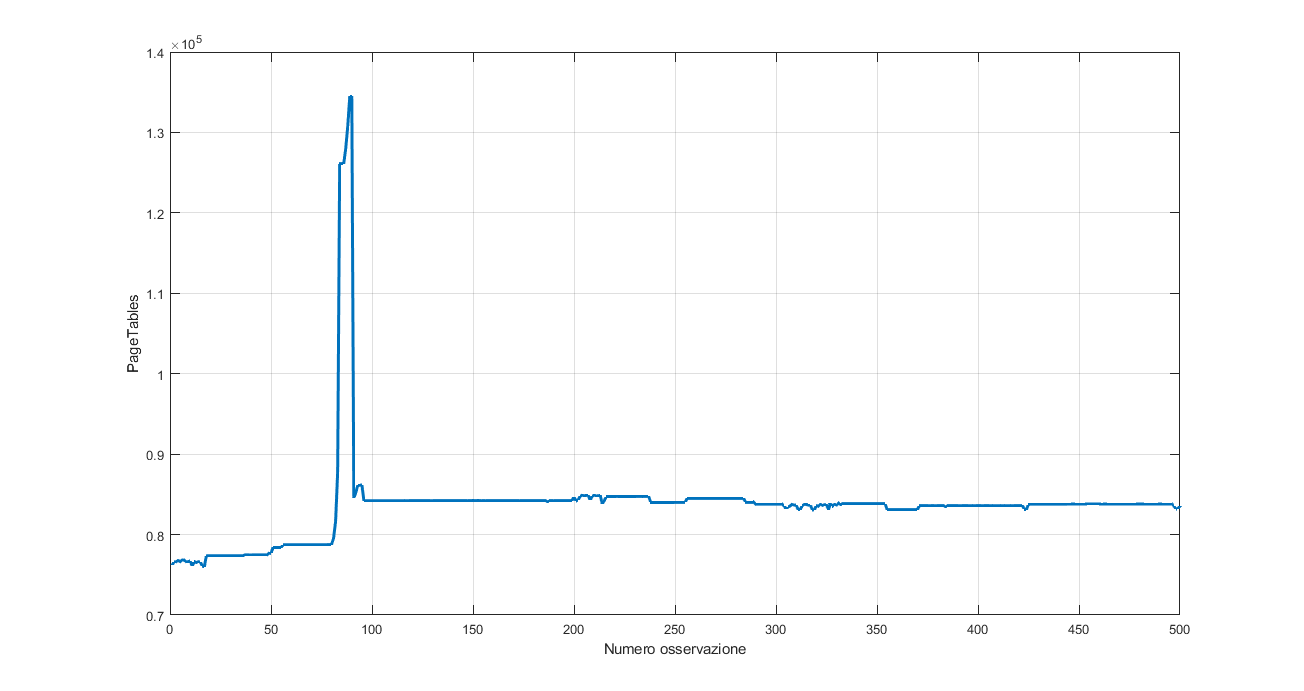
\includegraphics[width=\textwidth]{img/hw1/pagetables.png}}	
	\caption{\textit{Grafico tra numero di osservazione e valore assunto dal parametro PageTables}}
\end{figure}
Si nota che in corrispondenza (in realtà nell'osservazione appena precedente) dell'outlier del parametro \textit{Slab} i due parametri sopra indicati hanno un picco, durante la fase di avvio del sistema.
\\Lo Slab si riferisce ad un particolare meccanismo di allocazione/deallocazione della memoria nel Kernel. Dato che influenza in particolar modo altri parametri si è preferito non trascurarlo.\\
In conclusione sono stati eliminati dal dataset solo 2 outlier che corrispondono a 38 osservazioni. Quindi il dataset è stato ridotto in totale di 15.038 elementi, provocando una diminuzione dei dati iniziali di poco più del $20\%$.
\newpage

\section{PCA}
A seguito del filtraggio il dataset risulta ridotto grazie alla rimozione di alcune colonne che non esprimevano varianza e alcune righe rappresentanti outlier trascurabili.
\\Su questo dataset si possono quindi iniziare a fare le prime considerazioni.
\\Utilizzando la tecnica della \textit{Principal Component Analysis} il dataset può essere estremamente ridotto, sfruttando solo le \textit{Componenti Principali} che mantengono più varianza. Il risultato della PCA è quindi:
\begin{figure}[H]
	\centering
	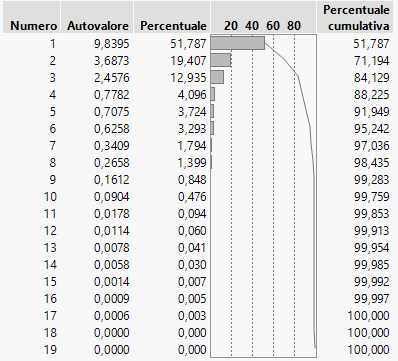
\includegraphics{img/hw1/pca.png}
	\caption{\textit{PCA applicata al dataset filtrato}}
\end{figure}
La scelta del numero di componenti principali ricade in particolar modo sulla devianza che quelle componenti mantengono rispetto al dataset reale. Inoltre essa dipende anche dal tipo di osservazioni ed esperimento che è stato effettuato.
\\In questo caso la scelta è ricaduta sul prendere 5 componenti principali poiché rappresentano il 92\% della devianza totale. Esso rappresenta un valore abbastanza elevato, ma è stato scelto per mantenersi in una regione di tolleranza durante la clusterizzazione. 
\\Anche se il workload sintentico verrà costruito considerando 5 componenti principali, in seguito sono riportati i risultati di PCA e clusterizzazione anche nel caso in cui fosse stato scelto un numero diverso di componenti principali, ovvero:
\begin{itemize}
	\item Prendere 4 PC
	\begin{equation*}
		DEV_{PCA-MANTENUTA} \approx 88 \%
	\end{equation*}
	\item Prendere 5 PC
	\begin{equation*}
			DEV_{PCA-MANTENUTA} \approx 92 \%
	\end{equation*}
	\item Prendere 6 PC
	\begin{equation*}
			DEV_{PCA-MANTENUTA} \approx 95 \%
	\end{equation*}
\end{itemize}
Per ognuno di questi 3 insiemi di Principal Components è stata effettuata la procedura di clustering .

\section{Clustering}
Il clustering è una tecnica che consiste nel raggruppare osservazioni "simili" tra loro. La similitudine tra un elemento e un cluster, o tra un cluster e un altro cluster, può essere calcolata secondo varie tecniche. In questa analisi si è preferito utilizzare il \textbf{metodo di Ward}, il quale pesa la distanza tra due cluster in relazione al numero di elementi che li compongono.
\\Dati due cluster P e Q (un elemento non appartenente ad un cluster, può essere visto come un cluster di dimensione 1), sia $|P|$ la cardinalità di $P$, analogo con $|Q|$, e sia $\bar{x}_p$ il centroide di $P$, analogo con $\bar{x}_q$, la distanza tra $P$ e $Q$ viene calcolata come:
\begin{equation*}
	d(P,Q) = 2 \dfrac{|P| \; |Q|}{|P| + |Q|} ||\bar{x}_p - \bar{x}_q ||^2
\end{equation*}
Per ogni raggruppamento viene poi scelto una singola osservazione che la rappresenta, riducendo quindi il numero di righe del dataset pari al numero di cluster scelti durante l'analisi.
\\Il numero di cluster da scegliere può dipendere da vari fattori:
\begin{itemize}
	\item Omogeneità dei cluster: i cluster devono raggruppare un numero di osservazioni quanto il più possibile omogeneo rispetto agli altri cluster. Avere un cluster con un numero di elementi di vari ordini di grandezza rispetto ad un altro cluster non sempre può portare a buoni risultati (in termini di devianza).
	\item Devianza mantenuta: a seguito della PCA parte della devianza nei dati viene persa. Dato che il clustering viene effettuato sulle \textit{Componenti Principali} allora esso produce un'ulteriore perdita di devianza nel risultato finale.
\end{itemize}
\subsubsection{Devianza Persa}
Per effettuare il calcolo della devianza totale persa persa bisogna prima calcolare la devianza intra-cluster (la somma delle devianze per ogni cluster) e sulla base di questa si può calcolare la quantità richiesta.
\\Matematicamente, definita $DEV_{PCA-PERSA}$ la devianza persa (in termini percentuali) a causa della PCA, viceversa $DEV_{PCA-MANTENUTA}$ la devianza mantenuta dalla PCA, e $DEV_{INTRA}$ la devianza intra-cluster, la devianza totale persa percentuale vale:
\begin{equation*}
	DEV_{PCA-LOST} + DEV_{INTRA}\times DEV_{PCA-MANTENUTA}
\end{equation*}
Essa può essere calcolata in MATLAB passando ad uno script i cluster, le componenti principali e il dataset iniziale.
\\ Per dare valore ai fattori sopra citati il clustering viene effettuato scegliendo un numero di cluster che varia da 6 a 16 (per ogni gruppo di componenti principali) su cui poi viene calcolata la devianza persa.
\newpage
 \subsection{4 Componenti Principali}
 Utilizzando le prime quattro PC si ha:
 \begin{figure}[H]
 	\centering   
 	\subfigure{	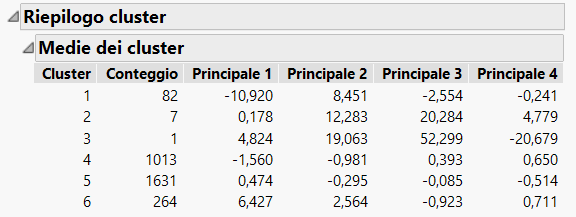
\includegraphics[width=0.30\textwidth]{Homework/Workload_Characterization/PCA_&_Clustering/4_Comp/Clustering/6_Cluster/Screen_Dati/Riepilogo.png}}
 	\subfigure{	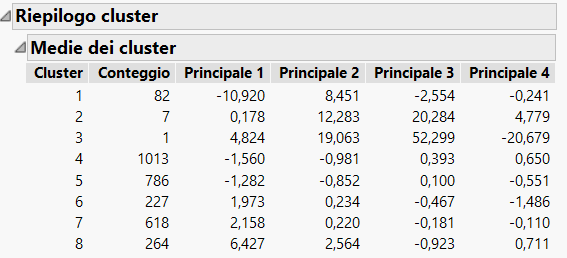
\includegraphics[width=0.30\textwidth]{Homework/Workload_Characterization/PCA_&_Clustering/4_Comp/Clustering/8_Cluster/Screen_Dati/Riepilogo.png}}
 	\subfigure{	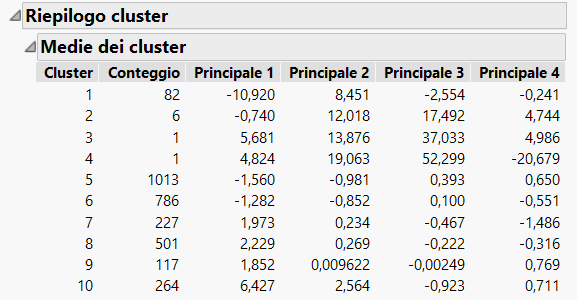
\includegraphics[width=0.30\textwidth]{Homework/Workload_Characterization/PCA_&_Clustering/4_Comp/Clustering/10_Cluster/Screen_Dati/Riepilogo.png}}
 	\subfigure{	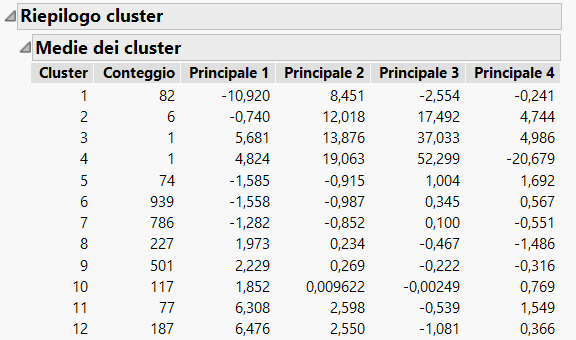
\includegraphics[width=0.30\textwidth]{Homework/Workload_Characterization/PCA_&_Clustering/4_Comp/Clustering/12_Cluster/Screen_Dati/Riepilogo.png}}
 	\subfigure{	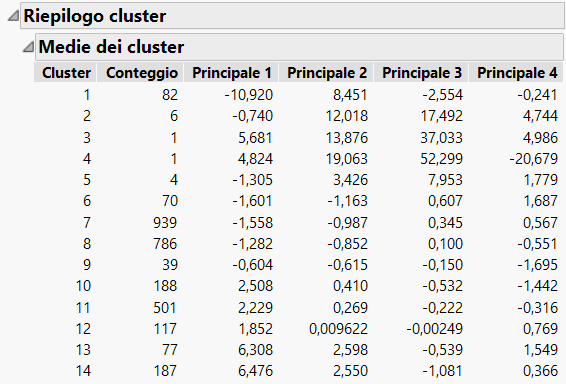
\includegraphics[width=0.30\textwidth]{Homework/Workload_Characterization/PCA_&_Clustering/4_Comp/Clustering/14_Cluster/Screen_Dati/Riepilogo.png}}
 	\subfigure{	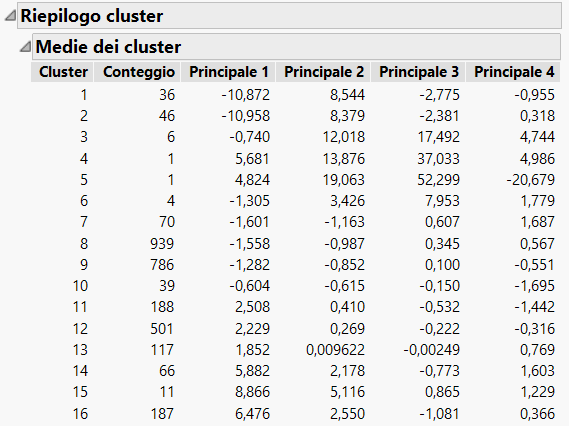
\includegraphics[width=0.30\textwidth]{Homework/Workload_Characterization/PCA_&_Clustering/4_Comp/Clustering/16_Cluster/Screen_Dati/Riepilogo.png}}
 	\caption{\textit{Numero di cluster e dimensione per diversi valori}}
 \end{figure}
La devianza persa durante la clusterizzazione varia in relazione al numero di cluster scelti. Si possono racchiudere le informazioni in un'unica tabella:
\begin{center}
	\begin{tabular}{|c|c|c|c|c|c|}
		\hline
		\textbf{6 Cluster} & \textbf{8 Cluster} & \textbf{10 Cluster} &\textbf{12 Cluster}& \textbf{14 Cluster} & \textbf{16 Cluster} \\
		\hline
		26\%& 17\% & 16\% & 15\% & 14.5\% & 14\% \\
		\hline
	\end{tabular}
\end{center}
\vspace{0.5cm}
 \subsection{5 Componenti Principali}
 Utilizzando le prime quattro PC si ha:
 \begin{figure}[H]
 	\centering   
 	\subfigure{	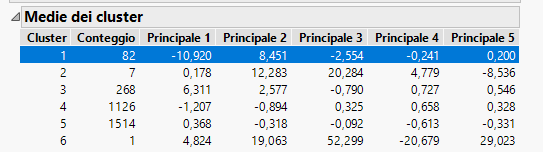
\includegraphics[width=0.30\textwidth]{Homework/Workload_Characterization/PCA_&_Clustering/5_Comp/Clustering/6_Cluster/Screen_Dati/Riepilogo.png}}
 	\subfigure{	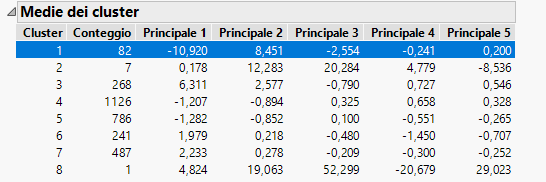
\includegraphics[width=0.30\textwidth]{Homework/Workload_Characterization/PCA_&_Clustering/5_Comp/Clustering/8_Cluster/Screen_Dati/Riepilogo.png}}
 	\subfigure{	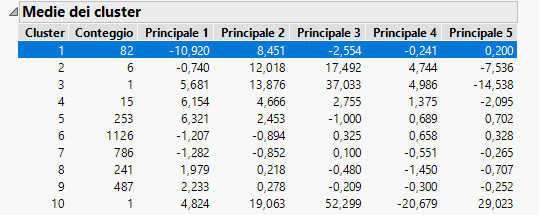
\includegraphics[width=0.30\textwidth]{Homework/Workload_Characterization/PCA_&_Clustering/5_Comp/Clustering/10_Cluster/Screen_Dati/Riepilogo.png}}
 	\subfigure{	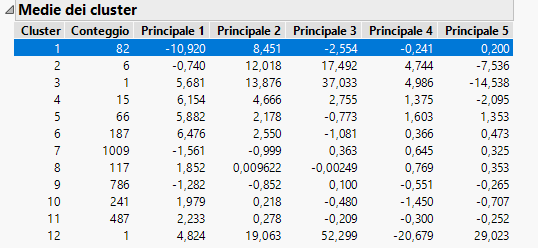
\includegraphics[width=0.30\textwidth]{Homework/Workload_Characterization/PCA_&_Clustering/5_Comp/Clustering/12_Cluster/Screen_Dati/Riepilogo.png}}
 	\subfigure{	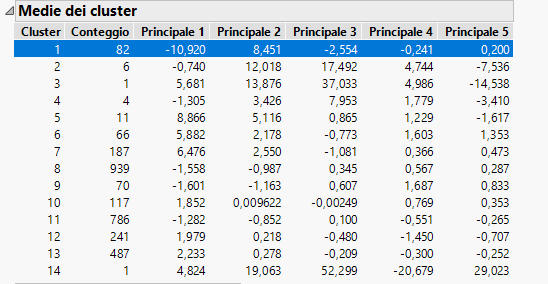
\includegraphics[width=0.30\textwidth]{Homework/Workload_Characterization/PCA_&_Clustering/5_Comp/Clustering/14_Cluster/Screen_Dati/Riepilogo.png}}
 	\subfigure{	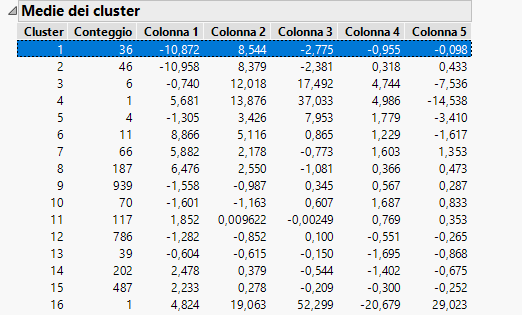
\includegraphics[width=0.30\textwidth]{Homework/Workload_Characterization/PCA_&_Clustering/5_Comp/Clustering/16_Cluster/Screen_Dati/Riepilogo.png}}
 	\caption{\textit{Numero di cluster e dimensione per diversi valori}}
 \end{figure}
La devianza persa durante la clusterizzazione varia in relazione al numero di cluster scelti. Si possono racchiudere le informazioni in un'unica tabella:
\begin{center}
	\begin{tabular}{|c|c|c|c|c|c|}
		\hline
		\textbf{6 Cluster} & \textbf{8 Cluster} & \textbf{10 Cluster} &\textbf{12 Cluster}& \textbf{14 Cluster} & \textbf{16 Cluster} \\
		\hline
		25.5\%& 16\% & 15\% & 12\% & 11\% & 10\% \\
		\hline
	\end{tabular}
\end{center}
\vspace{0.5cm}
 \subsection{6 Componenti Principali}
 Utilizzando le prime quattro PC si ha:
 \begin{figure}[H]
 	\centering   
 	\subfigure{	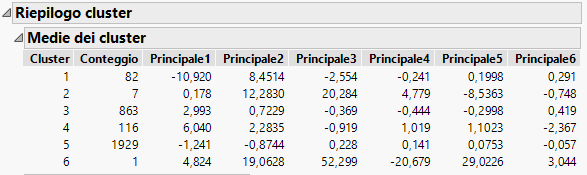
\includegraphics[width=0.30\textwidth]{Homework/Workload_Characterization/PCA_&_Clustering/6_Comp/Clustering/6_Cluster/Screen_Dati/Riepilogo.png}}
 	\subfigure{	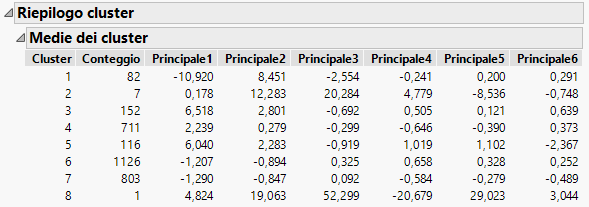
\includegraphics[width=0.30\textwidth]{Homework/Workload_Characterization/PCA_&_Clustering/6_Comp/Clustering/8_Cluster/Screen_Dati/Riepilogo.png}}
 	\subfigure{	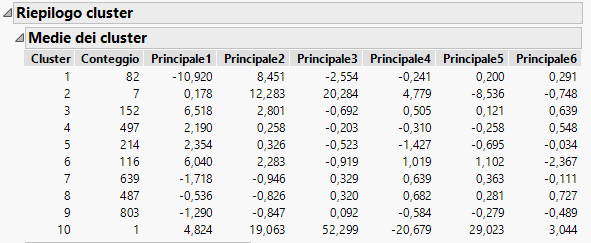
\includegraphics[width=0.30\textwidth]{Homework/Workload_Characterization/PCA_&_Clustering/6_Comp/Clustering/10_Cluster/Screen_Dati/Riepilogo.png}}
 	\subfigure{	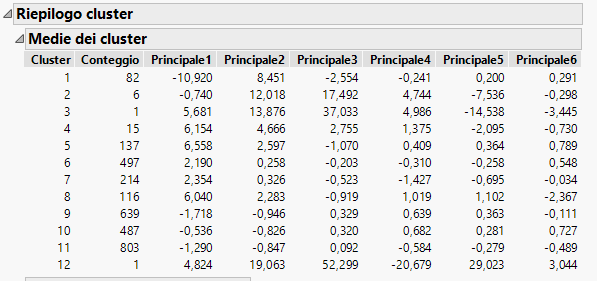
\includegraphics[width=0.30\textwidth]{Homework/Workload_Characterization/PCA_&_Clustering/6_Comp/Clustering/12_Cluster/Screen_Dati/Riepilogo.png}}
 	\subfigure{	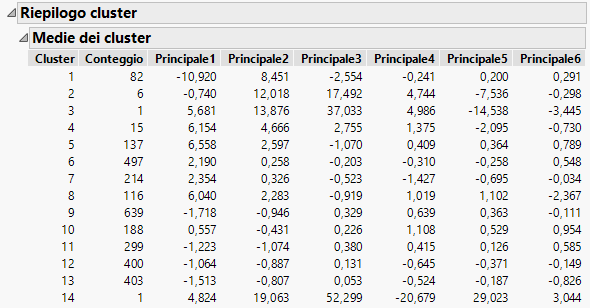
\includegraphics[width=0.30\textwidth]{Homework/Workload_Characterization/PCA_&_Clustering/6_Comp/Clustering/14_Cluster/Screen_Dati/Riepilogo.png}}
 	\subfigure{	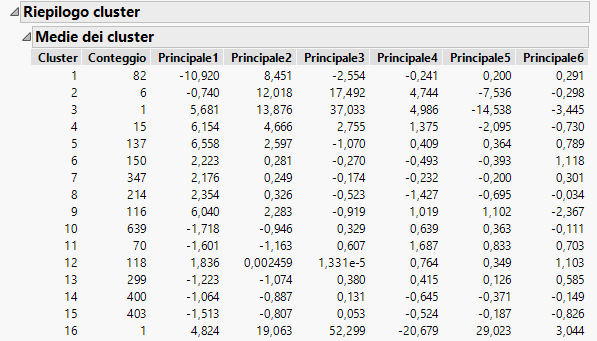
\includegraphics[width=0.30\textwidth]{Homework/Workload_Characterization/PCA_&_Clustering/6_Comp/Clustering/16_Cluster/Screen_Dati/Riepilogo.png}}
 	\caption{\textit{Numero di cluster e dimensione per diversi valori}}
 \end{figure}
 
 
 \begin{center}
 	\begin{tabular}{|c|c|c|c|c|c|}
 		\hline
 		\textbf{6 Cluster} & \textbf{8 Cluster} & \textbf{10 Cluster} &\textbf{12 Cluster}& \textbf{14 Cluster} & \textbf{16 Cluster} \\
 		\hline
 		22\% & 15\%& 13\% & 12\% & 11\% & 9\% \\
 		\hline
 	\end{tabular}
 \end{center}

\vspace{0.5cm}

\subsection{Interpretazione}
All'inizio dell'analisi sono state effettuate delle ipotesi che hanno trovato riscontro nella procedura di clustering:
\begin{enumerate}
	\item La fase iniziale del sistema (descritto dalle prime righe) trova riscontro con il cluster numero uno qualunque siano le componenti principali e qualunque sia il numero di cluster scelto. Questo quindi prova l'ipotesi definita inizialmente
	\item L'ultimo cluster contiene sempre un elemento singolo. Questo accade a causa del fatto che è stato identificato un picco nella fase iniziale delle misure. Esso inoltre è stato definito grazie all'outlier nel parametro Slab che non è stato eliminato, di conseguenza il picco viene racchiuso in un unico cluster in tutte le situazioni.
\end{enumerate}
\vspace{0.5cm}
In conclusione si può costruire una tabella che racchiude le informazioni riguardanti le PCA e la clusterizzazione in termini di percentuale di devianza persa.
 \begin{center}
	\begin{tabular}{|c|c|c|c|c|c|c|}
		\hline
		& \textbf{6 Cluster} & \textbf{8 Cluster} & \textbf{10 Cluster} &\textbf{12 Cluster}& \textbf{14 Cluster} & \textbf{16 Cluster} \\
		\hline
		\textbf{4 PC} & 26\%& 17\% & 16\% & 15\% & 14.5\% & 14\% \\

	\textbf{5 PC} & 25.5\%& 16\% & 15\% & 12\% & 11\% & 10\% \\

		\textbf{6 PC} & 22\% & 15\%& 13\% & 12\% & 11\% & 9\% \\
		\hline
	\end{tabular}
\end{center}

\newpage
\section{Workload Sintetico}
Come anticipato nel paragrafo precedente, sono state scelte 5 PC e per non perdere troppa varianza ma al tempo stesso non sfociare in un numero di cluster molto elevato, si è scelto di considerare 10 cluster. In tal caso la perdita di devianza con PCA e Cluster è di circa del 15\%.
\\In conclusione dopo aver calcolato i centroidi con uno script MATLAB il workload sintetico risulta essere:
\begin{figure}[H]
	\centering
	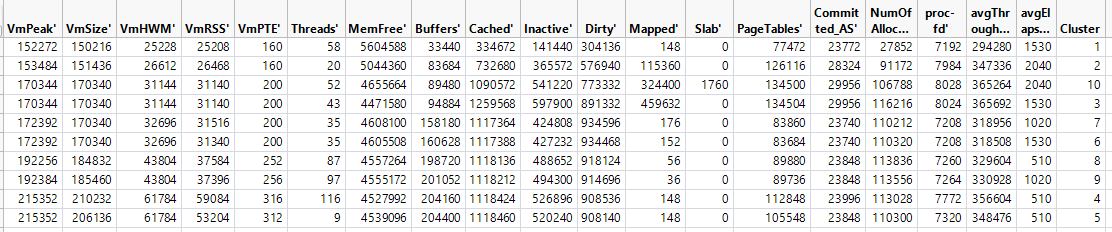
\includegraphics[width=\textwidth]{img/hw1/workload_sintetico.png}
	\caption{\textit{Workload sintetico}}
\end{figure}
	\chapter{Web Server - Capacity Test}
L'obiettivo del Capacity Test è quello di valutare le performance di un qualsiasi sistema quando è sottoposto a carichi di lavoro di diversa intensità, in modo da caratterizzare le sue prestazioni al limite (sotto condizioni di lavoro severe).
\\
Per realizzare queste valutazioni sono necessari gli \textbf{high-level parameters}, ovvero tutti quei parametri reperibili ed osservabili lato client. Essi possono riferirsi alla richiesta (quando è stata fatta, chi l'ha fatta ecc..) o alla risposta (tempi di risposta, errori).
\\
Essendo il sistema in questione un server, si è scelto di descrivere le sue performance attraverso:
\begin{enumerate}
	\item \textbf{Response Time}, intervallo di tempo che intercorre tra l'istante in cui il client inoltra la richiesta e quello in cui riceve la risposta.
	\item \textbf{Throughput}, richieste servite correttamente per unità di tempo.
\end{enumerate}
L'andamento atteso da parte di queste due metriche è il seguente:
\begin{figure}[H]
	\centering
	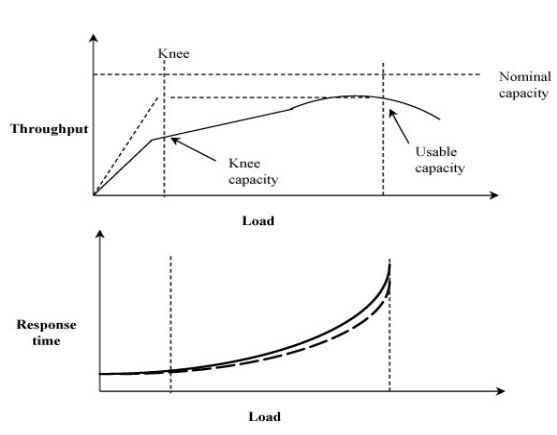
\includegraphics[width=0.8\textwidth]{img/hw2/Thr_resp.png}
	\caption{\textit{Grafici Throughput e Response time}}
\end{figure}
Di nostro interesse sono i valori di:
\begin{itemize}
	\item \textit{Knee Capacity}, punto prima del quale il throughput cresce linearmente all'aumentare del carico, ma il tempo di risposta non varia significativamente ed oltre il quale il guadagno in throughput è basso mentre il tempo di risposta aumenta con il carico.
	\item \textit{Usable Capacity}, massimo throughput raggiungibile portando il sistema al limite, senza eccedere un dato tempo di risposta.
\end{itemize}
Per ottenere agevolmente la Knee Capacity, viene introdotto un terzo parametro, la \textit{Potenza}. 
\\
\begin{equation}
	Power = \frac{Throughput}{Response Time}
\end{equation}
Tale punto coincide con il punto di massimo della potenza e rappresenta l'ottimo in corrispondenza del quale conviene operare per ottenere le prestazioni migliori.
\begin{figure}[H]
	\centering
	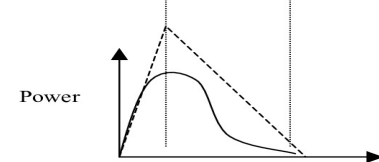
\includegraphics[width=0.5\textwidth]{img/hw2/Power.png}
	\caption{\textit{Grafico Potenza}}
\end{figure}


\section{Experimental Setup}
Il sistema oggetto di studio è un \textit{Web Server Apache} installato sulla macchina virtuale guest, che funge da server.
\\
Tramite la modalità \textit{Host-only Network Adapter}, configurabile nelle impostazioni della macchina virtuale, è stato possibile far comunicare la macchina guest con quella host, che lo ospita. Su quest'ultima è stata installata l'applicazione Java \textit{JMeter}, che ha permesso l'analisi delle prestazioni complessive del Server, sottoponendolo a diversi tipi di carico.
\\
\\
In questa analisi è stato scelto di valutare le prestazioni in media del server, considerando solo richieste (HTTP di tipo GET) casuali. Esse sono differenziate dalla dimensione della risorsa che chiedono al server. 

\subsection{Server Setup}
Il server è stato installato su una macchina virtuale \textit{Ubuntu 2021} in esecuzione su una macchina host di uso comune. Essa è stata dotata di circa 4GB di RAM e di 2 processori (intel I5-5200u con frequenza massima di 2.70 GHz).
\\Per creare un scenario reale, sul Server sono state caricate 5 pagine in formato testuale, di diversa dimensione:
\begin{itemize}
	\item \textbf{Small}: 50 KB
	\item \textbf{Small-Medium}: 100 KB
	\item \textbf{Medium}: 300 KB
	\item \textbf{Medium-Large}: 500 KB
	\item \textbf{Large}: 1 MB
\end{itemize}
Questi sono i file oggetto delle richieste realizzate da ipotetici client.

\subsection{Clients Setup - JMeter}
Innanzitutto è stato settato, nel \textit{ThreadGroup}, il numero di thread che JMeter usa per realizzare i test. Questa quantità rappresenta il numero di utenti "virtuali" che visitano il nostro server. Nel nostro esperimento sono stati previsti \textbf{50 threads}, un valore in linea con i suoi scopi (dato che si tratta di un banale webserver virtualizzato su una macchina host di uso comune). In più, prevedendo dei test di durata pari a \textit{5 min}, sono stati impostati:
\begin{itemize}
	\item il \textbf{Ramp-up period} - numero di secondi entro il quale deve essere attivato l'ultimo thread - a \textit{300 s}. Ciò ci ha permesso di dilazionare l'attivazione degli utenti nei 5 minuti.
	\item il \textbf{Thread lifetime} - durata massima di ogni thread - a \textit{300 s}.
	\item il \textbf{Loop count} - numero di volte in cui un singolo thread effettua una richiesta. Esso corrisponde al numero di richieste nell'intervallo di tempo di simulazione (in questo caso 300s) diviso il numero di threads.
\end{itemize}
Al ThreadGroup sono stati aggiunti 5 \textit{HTTP Request Sampler}, uno per tipologia di richiesta da realizzare e nei quali sono stati specificati i path delle rispettive risorse sul server. Ad essi è stato integrato un \textit{Random Controller}, grazie al quale, quando un thread viene attivato, effettua solo una tra le cinque tipologie di richieste, selezionata in maniera randomica. Ancora una volta, aggiungendo variabilità alle nostre richieste, è stato possibile simulare una situazione realistica e, soprattutto, non predicibile.
\\
Attraverso il \textit{Constant Throughput Timer} è stato possibile impostare il carico da sottoporre al sistema, in termini di numero di richieste al minuto. Infine, il listener \textit{Simple Data Writer}, ci ha permesso di collezionare in un file, quei parametri di alto livello che sono d'interesse ai fini dell'esperimento.
\\L'idea è quella di simulare quindi 50 utenti, di cui ognuno effettua un numero di richieste in relazione al carico, per 5 min. \\Ciò equivale a:
\begin{figure}[H]
	\centering
	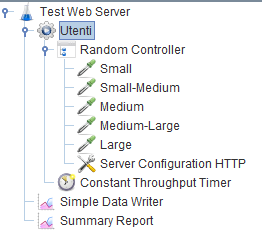
\includegraphics[width=0.4\textwidth]{img/hw2/jmeter.png}
	\caption{\textit{Configurazione delle richieste e del carico in JMeter}}
\end{figure}
I risultati, grazie al Simple Data Wirter, vengono salvati in formato .csv, i cui paramentri vengono raggruppati in forma tabellare.
\begin{center}
\begin{tabular}{|l|l|l|l|}
	\hline
	TimeStamp & Elapsed & Latency & ... \\
	\hline
	\vdots &  \vdots & \vdots & \vdots \\
	\hline
\end{tabular}
\end{center}
\section{Esecuzione Capacity Test}
Inizialmente sono stati effettuati dei test il cui scopo era quello di far operare il Web Server "al limite". Ci si è resi conto che il massimo valore di carico entro il quale il sistema risponde adeguatamente (in quelle condizioni), è di circa \textit{6000 richieste al minuto}. 
\\
A partire da questo limite e ragionando sull'andamento di throughput e response time, si sono scelti i seguenti valori di carico da sottoporre al sistema:
\begin{equation*}
	workloads = {100, 500, 800, 1000, 2000, 3000, 4000, 5000, 6000, 7000, 8000, 9000}
\end{equation*}
Gli ultimi tre carichi (7000, 8000 e 9000 richieste al minuto) hanno permesso di evidenziare nei grafici il degradamento delle prestazioni del sistema.
\\
Per ogni valore di carico è stato calcolato il \textbf{Throughput}:

\begin{equation}
	Throughput = \frac{NumeroRichieste}{Timestamp(N) - Timestamp(1)} \quad  \left[ \frac{N}{s} \right] 
\end{equation}
Il \textit{timestamp} fa parte degli high-level parameters collezionati dal Simple Data Writer, e corrisponde all'istante di tempo (in millisecondi poi convertito in secondi) in cui il client ha inoltrato una data richiesta.
\\
Come \textbf{Response Time} è stato scelto il parametro \textit{Elapsed}, coincidente con il tempo che intercorre tra la sottomissione della richiesta da parte del client e la risposta del server. Dato che contiene anche il tempo di elaborazione della richiesta da parte del server, esso cresce all'aumentare della dimensione dei file richiesti, oltre che all'aumentare del carico.
\\
\\
Ogni misurazione (per ogni carico) è stata ripetuta \textbf{3 volte} in modo da tenere traccia dell'errore, e notando che i dati ottenuti non differivano di molto tra loro, come indice di posizione è stata scelta la loro media.
\\
\subsection{Risultati}
I file .csv sono stati caricati in uno script Matlab tramite cui sono stati automatizzati i procedimenti descritti sopra, i parametri sono stati plottati in funzione del carico considerato.
differenziale).
\begin{minted}[framesep = 1mm,
	fontsize = \footnotesize,
	breaklines,
	]{MATLAB}
%% Data
workloads = [100 500 800 1000 2000 3000 4000 5000 6000 7000 8000 9000];
througputs = zeros(1, length(workloads));
resp_times = zeros(1, length(workloads));
k = 1; %Indice di riferimento per i due vettori

%% Elaborazione
for i = workloads
	mean_resp_t = zeros(1,3);
	thr = zeros(1,3);
	for j = 1:3
		path = strcat(num2str(i, '%d'),'\dati',num2str(j,'%d'),'.csv');
		
		%Data from Jmeter output file (csv format)
		simple_data = readmatrix(path);
		
		%Calculating the number of requests
		[N, M] = size(simple_data);
		num_req = N; %Number of requests
		
		%Throughput = number_of_requests_completed / time_window_of_the_experiment
		t_wind_mills = simple_data(num_req,1) - simple_data(1,1); %Time window (milliseconds)
		t_wind_sec = t_wind_mills/1000; %Time window (seconds)
		thr(j) = num_req/t_wind_sec; %Throughput
		
		%Average response time
		elap_times = simple_data(:,2);
		mean_resp_t(j) = mean(elap_times);
	end

	check deviazione_std    
	COV_thr(k) = std(thr)/mean(thr);
	COV_resp(k) = std(mean_resp_t)/mean(mean_resp_t);
	     
	if COV_thr(k) > 0.5     
		througputs(k) = median(thr);
	end

	if COV_resp(k) > 0.5
		resp_times(k) = median(mean_resp_t);
	end

end

power = througputs./(resp_times/1000);
power_max = max(power);
KNEE_CAPACITY = througputs(find(power == power_max));
\end{minted}
Effettuando un grafico dei risultati:
\begin{figure}[H]
	\centering
	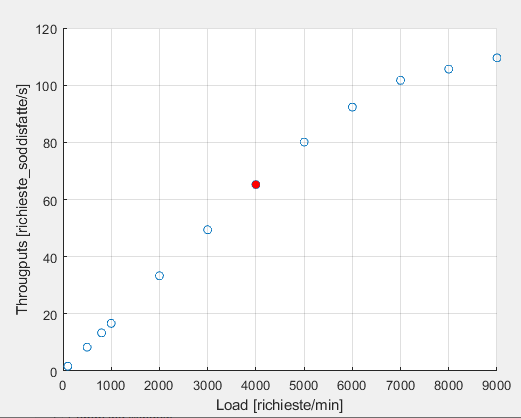
\includegraphics[width=0.8\textwidth]{img/hw2/Throughput.png}
	\caption{\textit{Grafico Throughput}}
\end{figure}

\begin{figure}[H]
	\centering
	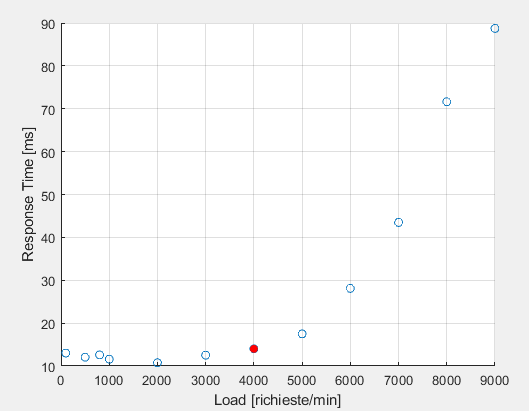
\includegraphics[width=0.8\textwidth]{img/hw2/ResponseTime.png}
	\caption{\textit{Grafico Response Time}}
\end{figure}

\begin{figure}[H]
	\centering
	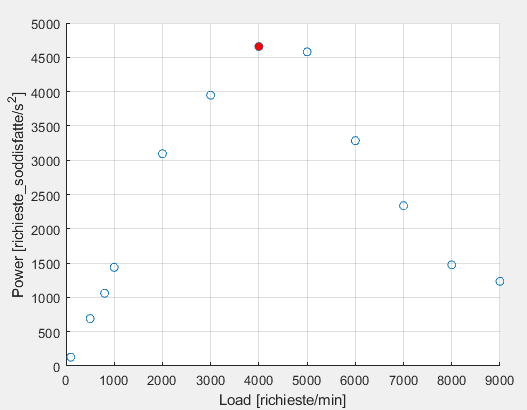
\includegraphics[width=0.8\textwidth]{img/hw2/Potenza.png}
	\caption{\textit{Grafico Potenza}}
\end{figure}
\newpage

Come si evince dal grafico della Potenza, il suo punto di massimo è associato ad un carico di 4000 richieste/min. 
\\
La \textit{Knee Capacity} (in rosso nel grafico dei Throughputs) è il valore throughput associato a questo carico. Ciò significa che se il nostro server opera in condizioni ottimali riesce a soddisfare circa 65,2112 richieste al secondo, ovvero 3836 richieste al minuto mediamente.
\\

Per quanto riguarda il calcolo della \textit{Usable Capacity}, possiamo relazionarla al tempo di risposta del server quando è sottoposto ad un carico di 6000 richieste/min (il carico limite). Questo response time è pari a 28,11 ms e coincide con quel tempo oltre il quale il sistema inizia a non rispondere più adeguatamente. Pertanto, la Usable Capacity può essere espressa come il valore di throughput associato al carico limite, ovvero 92,3314 richieste al secondo (5431 richieste al minuto circa).
\\
Ovviamente il valore di carico a cui conviene far lavorare il nostro Web Server non è quello massimo che riesce a soddisfare (Usable Capacity). Difatti non sarebbe efficiente per due motivi:
\begin{enumerate}
	\item I tempi di risposta associato a tale carico sono elevati.
	\item Essendo il carico limite, bastano poche richieste in più per ricadere nella zona in cui i tempi di risposta diventano estremamente elevati, rendendo inutilizzabile il server stesso. 
\end{enumerate}

	\chapter{Web Server - Workload Characterization}
L'obiettivo dell'homework è quello di realizzare un workload sintetico semplice e ripetibile, sulla base di un workload reale, attraverso le tecniche descritte nei capitoli precedenti. Successivamente esso deve essere applicato al sistema e, infine, si deve dimostrare che statisticamente si ottiene lo stesso risultato di un workload reale. L'esperimento può essere descritto in tre fasi:
\begin{enumerate}
	\item \textit{Simulazione di un workload reale}. In questa fase si simulano delle richieste random con carico prefissato al sistema. Si collezionano quindi i dati del client (lista delle richieste) di "alto livello" e i dati del server (memoria, utilizzo della CPU, ecc.) di "basso livello". Alla fine di questa fase bisogna analizzare i dati di alto livello per costruire un workload sintetico.
	\item \textit{Applicazione di un workload sintetico}. Dopo aver ricavato il workload sintetico al termine della fase precedente, esso deve essere applicato al sistema. Nuovamente quindi devono essere collezionati i dati di alto livello e basso livello.
	\item \textit{Validazione dei dati}. Prevede un'analisi approfondita dei dati di basso livello del workload reale e sintetico. Essi devono essere oppurtunamente caratterizzati per essere infine confrontati statisticamente. Per farlo si utilizzano dei test statistici meglio descritti successivamente.
\end{enumerate}
Le tre fasi possono essere rappresentate graficamente come nella successiva figura.

\begin{figure}[H]
	\centering
	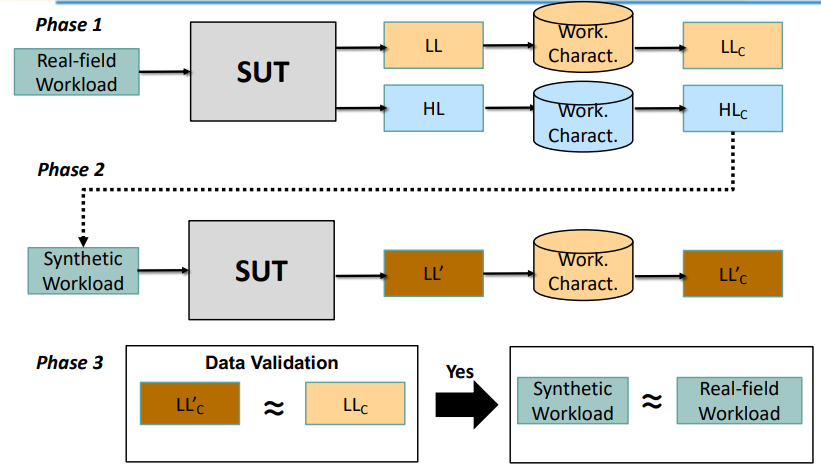
\includegraphics[width=0.6\textwidth]{img/hw3/Overview.png}
	\caption{\textit{Overview WL Characterization}}
\end{figure}

Per tutte le fasi il server occorre configurarlo allo stesso modo. In particolare si è utilizzato lo stesso Web Server descritto nel \textit{Capitolo 2} ma con una diminuzione di prestazioni solo a scopo didattico.

\section{Real-field Workload}
Per simulare quanto il più possibile un workload reale. Inoltre i dati di alto e basso livello devono essere presi contemporaneamente nel client e nel server.
\subsection{Server}
Il server contiene 10 file di diversa dimensione. I file sono stati scelti tutti dello stesso tipo (file di testo) solo per dimensionarli a piacimento. Nulla vieta però di utilizzare file di tipologie diverse (immagini, documenti, audio, etc.).
\\Essi sono stati dimensionati differenziando i file tra loro di 50 KB e partendo da un minimo di 50 KB.

\subsubsection{Parametri di basso livello}
Il web server è una macchina virtuale linux. Esistono dunque molti tool in grado di collezionare i parametri di caratteristici del sistema. In questo caso è stato utilizzato il tool \textbf{vmstat} (\textbf{Virtual memory statistics reporter}) il quale fornisce informazioni circa le performance del sistema su cui viene eseguito. In particolare esse riguardano:
\begin{itemize}
	\item \textbf{Processi}: numero processi in esecuzione o in attesa di essere eseguiti.
	\item \textbf{Memoria}:
		\begin{enumerate}
			\item \textit{free}, quantità di memoria libera.
		\end{enumerate}
	\item \textbf{Swap}
	\item \textbf{Input/Output}: blocchi ricevuti o inviati da/verso un dispositivo a blocchi.
	\item \textbf{Sistema}: 
		\begin{enumerate}
			\item \textit{in}, numero di interruzioni al secondo.
			\item \textit{cs}, numero di cambi di contesto al secondo.
		\end{enumerate}
	\item \textbf{CPU}: 
		\begin{enumerate}
			\item \textit{us}, tempo trascorso dalla CPU nell'eseguire codice non-kernel
			\item \textit{sy}, tempo trascorso dalla CPU nell'eseguire codice kernel
			\item \textit{id}, tempo trascorso dalla CPU nello stato di idle
		\end{enumerate}
\end{itemize}
Tali informazioni sono tutte utili ai fini dell'esperimento, ma quelle che evidenziano maggiormente gli effetti della nostra analisi sono quelle relative alla CPU e all'I/O.
\\
Vmstat offre inoltre la funzionalità di eseguire un campionamento dei parametri ad una frequenza e durata prefissata, tramite l'apposito comando eseguibile da terminale:
\begin{minted}[framesep = 1mm,
	fontsize = \footnotesize,
	breaklines,
	]{PYTHON}
	vmstat -n 1 400
\end{minted}
Il primo parametro "1" indica il periodo di campionamento in secondi, mentre il secondo parametro "400" indica la durata totale di esecuzione in secondi. L'output poi può essere semplicemente salvato in un file di testo o csv.
\\
Tale comando è stato avviato pochi secondi prima dell'avvio del test su Jmeter, ed ha continuato a campionare per qualche secondo anche dopo la sua fine, dunque nell'analisi dei dati sono attesi parametri il cui andamento evidenzia le varie fasi.


\subsection{Client - JMeter}
La simulazione degli utenti che fanno accesso al server è stata possibile tramite il tool JMeter, già descritto nei capitoli precedenti. 
\\In particolare sono stati realizzati tre Thread Group ognuno composto da 10 Thread (l'equivalente di 10 utenti) con una durata di simulazione pari a 2 min ciascuno. Ogni gruppo contiene 10 richieste riferite alle 10 risorse disponibili nel web server. Esse vengono poi eseguite in modo casuale tramite un apposito controller. 
\begin{figure}[H]
	\centering
	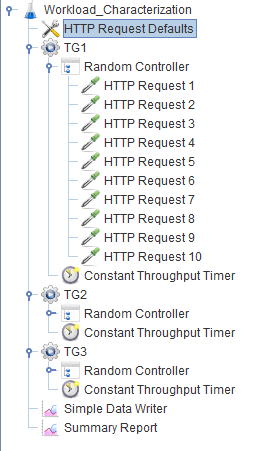
\includegraphics[width=0.4\textwidth]{img/hw3/jmeter_reale.png}
	\caption{\textit{Configurazione di JMeter per la simulazione di un workload reale}}
\end{figure}
Ogni gruppo inoltre ha un suo specifico carico. In questo caso si ha:
\begin{itemize}
	\item \textbf{TG1} : 400 richieste al minuto
	\item \textbf{TG2} : 550 richieste al minuto
	\item \textbf{TG3} : 700 richieste al minuto
\end{itemize}
Essi vengono poi eseguiti in sequenza e non in parallelo. Questo perché si possono creare possibili conflitti sulle risorse, dati dal fatto che ogni gruppo richiede le stesse risorse degli altri. 
\subsubsection{Parametri di alto livello}
I parametri di alto livello possono essere collezionati direttamente tramite il tool JMeter e salvati in formato \textit{.cvs}. Non sono necessari dunque programmi esterni. I parametri utili ai fini dell'analisi sono:
\begin{itemize}
	\item \textbf{Timestamp}, l'istante di tempo in cui viene effettuata la corrispettiva richiesta (in millisecondi)
	\item \textbf{elapse}, inteso come Response Time
	\item \textbf{label}, contiene l'informazione categorica della richiesta effettuata.
	\item \textbf{bytes}, numero di byte ricevuti tramite la relativa richiesta.
	\item \textbf{sentBytes}, numero di byte inviati per effettuare la richiesta.
	\item \textbf{latency}
	\item \textbf{connect}, tempo di connessione misurato per effettuare l'handshake TCP (in millisecondi).
\end{itemize}

\subsection{Workload Characterization}
Le misure vengono effettuate correttamente avviando prima \textit{vmstat} nel server e in seguito JMeter sul client in modo che i dati vengono salvati contemporaneamente nel lato client (alto livello) e nel lato server (basso livello). Al termine della simulazione quindi ci si ritrovano due file di dati.

\subsubsection{Parametri di alto livello}
I parametri di alto livello vanno incontro alla procedura di filtraggio, PCA e Clustering per ridurne la dimensionalità.
\\Essi appaiono nel seguente modo:
\begin{figure}[H]
	\centering
	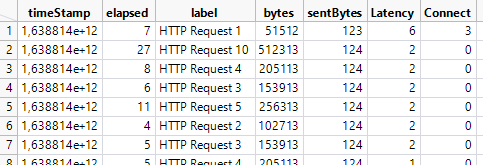
\includegraphics[width=0.8\textwidth]{img/hw3/alto_livello_esempio.png}
	\caption{\textit{Parametri di alto livello utili ai fini dell'analisi}}
\end{figure}
\hrule
\vspace{0.3cm}
La fase di filtraggio non prevede nessuna azione di modifica del dataset.
\\Sul dataset originale quindi deve essere effettuata la PCA per cercare di ridurne la dimensionalità senza perdere troppa varianza. Bisogna soprattutto considerare che per questi parametri la fase di Clustering è molto importante poiché racchiude le informazioni principali per costruire il workload sintetico.
\vspace{0.3cm}
\hrule
\vspace{0.3cm}
Tramite la PCA sono state scelte tutte le componenti principali, mantenendo una varianza del 100\%.
\begin{figure}[H]
	\centering
	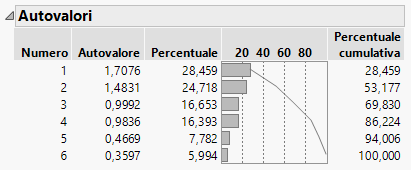
\includegraphics[width=0.6\textwidth]{img/hw3/autovalori.png}
	\caption{\textit{Analisi della varianza tramite autovalori}}
\end{figure}
Sulla base di queste può essere effettuato il clustering gerarchico.
\vspace{0.3cm}
\hrule
\vspace{0.3cm}
Il numero di cluster rappresenta il numero di richieste del workload sintetico, poiché in ogni cluster viene scelto un elemento rappresentativo di esso stesso. A tal proposito quindi il numero di cluster non deve essere maggiore del numero di \textit{HTTP Request} totali utilizzate durante la simulazione (in questo caso 30) e non deve essere un numero molto elevato. Al tempo stesso però non si deve perdere molta varianza a causa della clusterizzazione. 
\\La via più semplice è quella di effettuare delle prove scegliendo un numero di cluster minore della metà (in questo caso minore di 15) e valutare per ogni numero quanta varianza si perde.
\\Partendo da 6 componenti principali si può scegliere un numero di cluster variabile e calcolare la devianza persa per ogni valore.
\begin{center}
	\begin{tabular}{|c|c|c|c|c|c|}
		\hline
		\textbf{6 Cluster} & \textbf{8 Cluster} & \textbf{10 Cluster} &\textbf{12 Cluster} \\
		\hline
		35\% & 27\%& 21.5\% & 17\% \\
		\hline
	\end{tabular}
\end{center}
La scelta ricade su 10 cluster in modo da avere un workload sintetico abbastanza ristretto e una perdita di varianza non troppo elevato.
\\Per scegliere gli elementi rappresentativi di un cluster si può ricorrere a vari metodi:
\begin{itemize}
	\item Il punto più centrale possibile
	\item Il punto in cui un valore categorico si ripete più volte. Applicabile però solo se il dataset ha un parametro categorico in un insieme limitato di valori.
	\item Casualmente
	\item Il punto che si avvicina il più possibile alla media del cluster
	\item Etc.
\end{itemize}

\subsubsection{Parametri di basso livello}
\begin{figure}[H]
	\centering
	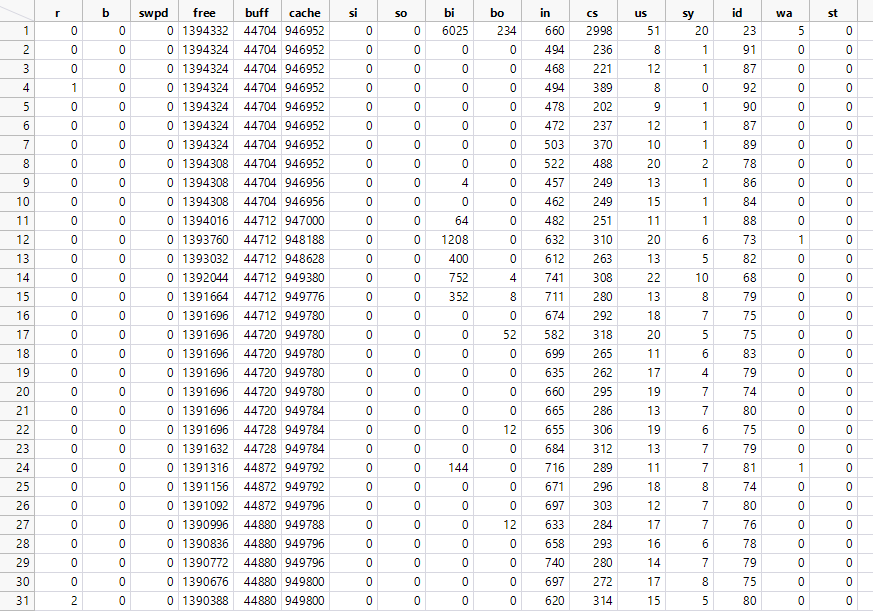
\includegraphics[width=0.7\textwidth]{img/hw3/porzione_lowlevel.png}
	\caption{\textit{Porzione dataset - Low Level Parameters}}
\end{figure}
I parametri di basso livello costituiscono un dataset formato da 17 colonne e 400 righe. Su di esso sono state dunque effettuate operazioni di \textit{filtraggio}, \textit{PCA} e \textit{clustering}, procedendo in maniera analoga a quanto già si era fatto nel Capitolo 1.
\\
\hrule
\vspace{0.3cm}
Analizzando le distribuzioni sono state individuate 4 colonne costanti (e quindi da rimuovere): \textbf{swpd}, \textbf{si}, \textbf{so}, \textbf{st}.
\\
Dopodichè sono state eliminate tutte le righe associate ai campioni prelevati da vmstat quando il client non stava sottoponendo richieste al server, in quanto non forniscono informazioni utili agli scopi della caratterizzazione.
\\
Per fare ciò sono stati analizzati gli andamenti in funzione del tempo dei parametri relativi all'utilizzo della CPU precedentemente descritti.
\begin{figure}[H]
	\subfigure{	
		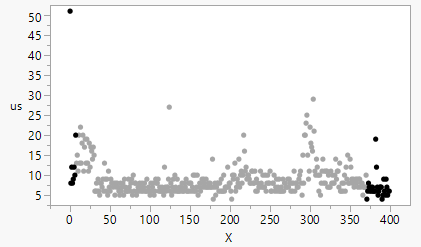
\includegraphics[width=0.30\textwidth]{img/hw3/us.png}}
	\subfigure{	
		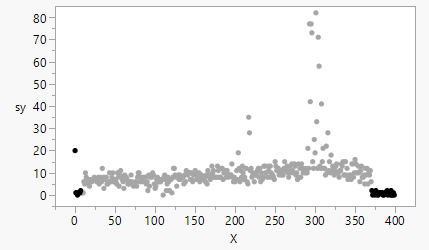
\includegraphics[width=0.30\textwidth]{img/hw3/sy.png}}
	\subfigure{	
		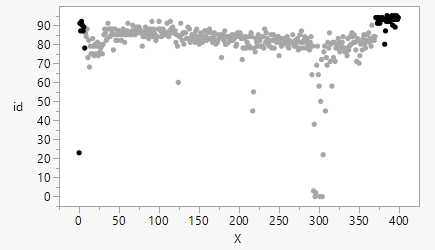
\includegraphics[width=0.30\textwidth]{img/hw3/id.png}}
	\caption{\textit{Andamento parametri CPU}}
\end{figure}
In particolare, osservando i grafici di \textit{sy} e \textit{id} risultano evidenti queste "fasi" nelle quali il processore trascorre meno tempo ad eseguire codice kernel e più tempo in idle rispetto a quando si sta sottoponendo il workload, visto che non è impegnato nel servire le richieste.
\\
Discorso analogo lo si può fare osservando le interruzioni al secondo (\textbf{in}), che incrementano drasticamente nel corso della recezione delle richieste, per poi diminuire in queste fasi.
\begin{figure}[H]
	\centering   
	\subfigure{	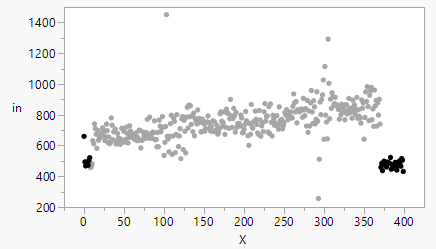
\includegraphics[width=0.30\textwidth]{img/hw3/interrupts.png}}
	\subfigure{
		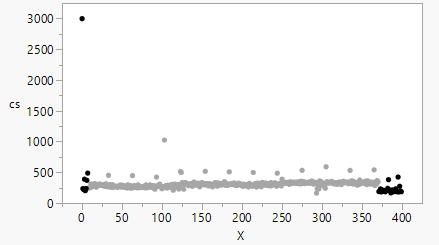
\includegraphics[width=0.30\textwidth]{img/hw3/cs1.png}}
	\caption{\textit{Andamento parametri di Sistema e CPU}}
\end{figure}
Contestualmente è stata eliminata anche la prima riga (outlier per quasi tutti i parametri), in quando è stata associata alla fase di avvio dell'esecuzione del comando vmstat e quindi non di particolare interesse per gli scopi dell'esperimento.
\\
L'ultima operazione effettuata in questa prima fase di filtraggio è stata la rimozione di un outlaier associato al parametro \textbf{b}, il quale è indice del numero di processi sospesi ed in attesa di risorse per poter essere riattivati.
Essendo outlaier anche di \textbf{wa} (tempo trascorso dalla CPU in attesa di input/output) è quasi sicuramente indice dello stesso fenomeno, il quale è stato da noi considerato come casuale e quindi trascurabile.
\begin{figure}[H]
	\centering
	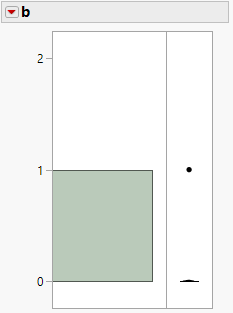
\includegraphics[width=0.3\textwidth]{img/hw3/outlaier_b.png}
	\caption{\textit{Distribuzione di b}}
\end{figure}
La riga ad esso associata è la 122, la quale è stata opportunamente rimossa. A seguito di questa cancellazione, la colonna associata al parametro b è diventata costante ed è dunque stata eliminata.
\\
\hrule
\vspace{0.3cm}
Il dataset ottenuto è formato da 12 colonne e circa 360 righe. Il numero di righe risultante può essere ulteriormente validato se consideriamo che la durata del test è proprio di 360 secondi.
\\
\\
Su questi dati è stata effettuata la PCA, a seguito della quale sono state prese in considerazione \textit{7 componenti principali}, le quali spiegano il 92,768 \% della devianza totale.
\begin{figure}[H]
	\centering
	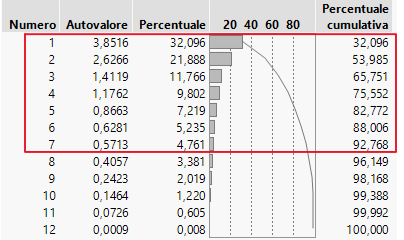
\includegraphics[width=0.5\textwidth]{img/hw3/PCA7.png}
	\caption{\textit{PCA Low-Level Filtered}}
\end{figure}
\hrule
\vspace{0.3cm}
Per non perdere una porzione significativa di devianza, dopo vari test, si è deciso di selezionare \textbf{20 Cluster} conservandone il 78,36\%.
\\
Infine è stata implementata in Matlab la seguente funzione per scegliere l'elemento rappresentativo di ogni cluster:
\begin{minted}[framesep = 1mm,
	fontsize = \footnotesize,
	breaklines,
	]{MATLAB}
	function [new_workload] = random_selection(workload)
	%workload = colonne PCA + colonna cluster
	N_cluster = max(workload(:,end)); %numero cluster
	[r,c] = size(workload);
	
	%isolo la colonna dei cluster
	cluster_data = workload(:,end);
	
	new_workload = zeros(N_cluster,c);
	
	%itero per ogni cluster
	for i = 1:N_cluster
	%prelevo tutti gli indici di riga associati ad uno stesso cluster i
		index = find(cluster_data==i); 
		%se ho più di una riga ne scelgo una random
		if length(index) > 1
			new_workload(i,:) = workload(randsample(index,1),:); 
		else
			%se ho solo una riga scelgo quella
			new_workload(i,:) = workload(index,:);
		end
	end
	end
\end{minted}
La funzione riceve in input le colonne estratte dalla PCA affiancate alla colonna dei cluster, la quale specifica il cluster di appartenenza di ciascuna riga.
Come si evince dal codice, i centroidi sono stati selezionati in maniera randomica nel caso in cui nel cluster sia presente più di un elemento.
\\
L'output della funzione è un workload costituito da 7 colonne e 20 righe, rappresentativo di quello originario.

\section{Synthetic Workload}
A partire dalla clusterizzazione di alto livello, identificati gli elementi rappresentativi di ogni cluster, si deve rifare la simulazione ma con il workload sintetico.
\\Il dataset in esame è composto da un parametro categorico che rappresenta la richiesta effettuata (risorsa e utente) facendo parte di un insieme molto limitato. La scelta può quindi ricadere sulla seconda possibilità.
\\A tal proposito si può calcolare una tabella che per ogni cluster indica il numero di ricorrenze del valore del parametro categorico.
\begin{figure}[H]
	\centering
	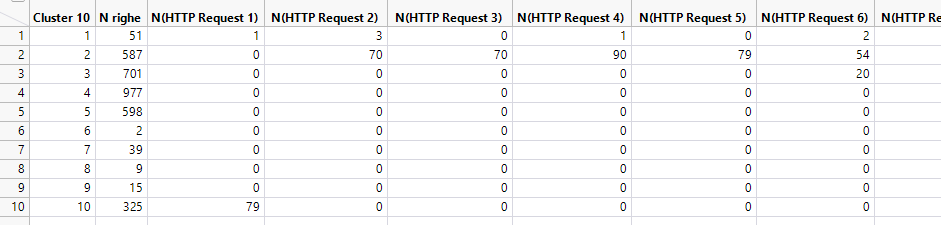
\includegraphics[width=\textwidth]{img/hw3/cluster_label.png}
	\caption{\textit{Tabella che associa ad ogni cluster il numero di punti con una determinata \textit{label}}}
\end{figure}
La matrice che compone la tabella è una matrice 10x30 e bisogna calcolare il massimo di riga per ogni riga. Inoltre se il massimo di riga è associato ad una \textit{label} già selezionata in precedenza, allora si deve scegliere il secondo massimo nella riga e così via. Si può automatizzare il tutto tramite uno script MATLAB:
\begin{minted}[framesep = 1mm,
	fontsize = \footnotesize,
	breaklines,
	]{MATLAB}
%% Dati
[data, txt] = xlsread('label-cluster 10');
data_filter = data(:, 3:end); 
txt_filter = txt(:, 3:end)';

%% Ricerca centroidi
[r,c] = size(data_filter);
max_list = zeros(1,r);  % Lista dei massimi
max_index = zeros(1,r); % Lista degli indici dei massimi

%Inizializzo vettore degli indici
for i=1:r
	max_index(i) = -1;
end

for i=1:r
	[temp_v, temp_i] =  max(data_filter(i,:));
	while ismember(temp_i,max_index)
		data_filter(i,temp_i) = -1;
		[temp_v, temp_i] =  max(data_filter(i,:));
	end
	max_list(i) = temp_v;
	max_index(i) = temp_i;
end

%% Stampa risultati
sort(txt_filter(max_index))
\end{minted}
Il risultato dello script è la lista delle \textit{label} che identificano il workload sintetico.
\begin{enumerate}
	\item HTTP Request 1 : TG1 con risorsa \textit{200k.txt}
	\item HTTP Request 11 : TG2 con risorsa \textit{50k.txt}
	\item HTTP Request 17 : TG2 con risorsa \textit{350k.txt}
	\item HTTP Request 21 : TG3 con risorsa \textit{50k.txt}	
	\item HTTP Request 22 : TG3 con risorsa \textit{100k.txt}		
	\item HTTP Request 23 : TG3 con risorsa \textit{150k.txt}		
	\item HTTP Request 25 : TG3 con risorsa \textit{250k.txt}		
	\item HTTP Request 27 : TG3 con risorsa \textit{350k.txt}
	\item HTTP Request 28 : TG3 con risorsa \textit{400k.txt}			
	\item HTTP Request 29 : TG3 con risorsa \textit{450k.txt}		
\end{enumerate}

\subsection{Server}
Il server non deve essere assolutamente modificato. Tutte le configurazioni effettuate per il workload reale rimangono invariate

\subsubsection{Parametri di basso livello}
I parametri di basso livello devono essere collezionati allo stesso modo utilizzato nel workload reale. Essi devono essere confrontati con i parametri di basso livello salvati durante la simulazione del workload reale. Questa operazione verrà analizzata nel paragrafo \textit{Data Validation}.

\subsection{Client - JMeter}
Il client deve, a questo punto, simulare le nuove richieste applicando il workload sintetico ricavato con l'analisi. Anche in questo caso la configurazione di JMeter non deve essere modificata, tranne che per le richieste.
\begin{figure}[H]
	\centering
	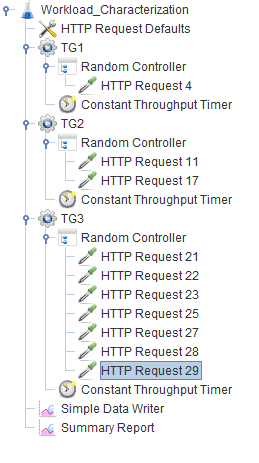
\includegraphics[width=0.4\textwidth]{img/hw3/jmeter_sintetico.png}
	\caption{\textit{Configurazione di JMeter per il workload sintetico}}
\end{figure}

\subsubsection{Parametri di alto livello}
I parametri di alto livello possono anche non essere collezionati poiché non servono per ulteriori analisi. Per completezza però si possono salvare tramite lo stesso JMeter usato per la simulazione.


\subsection{Workload Characterization}
\subsubsection{Parametri di basso livello}
Anche in questo caso il dataset di basso livello è costituito da 17 colonne e 400 righe. Analogamente a quanto fatto in precedenza per i parametri relativi al Workload reale sono state eseguite le operazioni di filtraggio, PCA e clustering.
\\
Sono state eliminate le colonne costanti, che in questo caso sono: \textbf{b}, \textbf{swpd}, \textbf{si}, \textbf{so} e \textbf{st}.
\\
Dopodichè, eliminando le righe relative ai campionamenti nelle fasi in cui il sistema non stava servendo alcuna richiesta, il set di dati è stato ulteriormente ridotto. L'analisi degli outlaier non ha portato all'eliminazione di alcuna riga, in quanto tutti i punti oltre i quartili dei box-plot sono stati considerati significativi. 
\\
\hrule
\vspace{0.3cm}
Come accaduto anche in precedenza, il dataset risultate è composto da 12 colonne e circa 360 righe (coerentemente con il tempo di sottomissione del workload).
\\
\begin{figure}[H]
	\centering
	\includegraphics[width=0.5\textwidth]{img/hw3/PCA7_syn.png}
	\caption{\textit{PCA syn Low-Level Filtered}}
\end{figure}
Per la PCA è stato scelto lo stesso numero di componenti selezionate nella caratterizzazione dei parametri di basso livello del workload reale.
Questa è stata una scelta obbligata dal fatto che le funzioni Matlab utilizzate per la validazione operano su matrici le quali devono necessariamente avere lo stesso numero di colonne.
\\
In ogni caso selezionando tali componenti si riesce a mantenere un'ottima percentuale di devianza: il 93,279\%.
\\
\hrule
\vspace{0.3cm}
Anche qui la scelta più conveniente in termini di devianza persa è stata quella di suddividere il dataset in 20 Cluster, conservandone il 75,51\% della totale. 
\\
Infine il workload di basso livello così ottenuto, è stato dato in input alla funzione \textit{random\_selection}, già descritta in precedenza, per ricavare i centroidi di ogni cluster.
\section{Data Validation}
I parametri di basso livello relativi a workload reale e sintetico, ottenuti in seguito alla caratterizzazione sono i seguenti:
\begin{figure}[H]
	\centering
	\includegraphics[width=0.6\textwidth]{img/hw3/real_wl.png}
	\caption{\textit{Low-Level Parameters Real WL}}
\end{figure}
\begin{figure}[H]
	\centering
	\includegraphics[width=0.6\textwidth]{img/hw3/syn_wl.png}
	\caption{\textit{Low-Level Parameters Synthetic WL}}
\end{figure}
Sono questi che andranno statisticamente confrontati per validare il Workload Sintetico.
\\La procedura per la validazione è molto semplice:
\begin{enumerate}
	\item Normalità verificata. Se i due dataset provengono da una distribuzione normale allora si possono eseguire test parametrici per la validazione. In particolare si possono usare vari tipi di test statistici anche in base all'omoschedasticità dei campioni.
	\begin{enumerate}
		\item Omostedasticità verificata. Se i due dataset sono omoschedastici allora si possono utilizzare test sulla base di questa condizione verificata.
		\item Omoschedasticità non verificata. Se i due dataset non rispettano la proprietà di omoschedasticità allora bisogna utilizzare test che si basano su tale condizione non verificata.
	\end{enumerate}
	\item Nomarlità non verificata. Se i due dataset non provengono da una distribuzione normale allora si devono usare necessariamente test statistici non parametrici per la validazione.
\end{enumerate}

\subsection{Normalità}
Per verificare se un campione proviene da una popolazione con distribuzione normale, ci si può affidare a test visivi oppure a test statistici analitici.
\subsubsection{Test Visivo}
Visivamente si può capire se un campione proviene da una popolazione con distribuzione normale effettuando un grafico dei quantili del campione rispetto ai quantili di una distribuzione normale. Ciò lo si realizza sfruttando la funzione Matlab \textbf{qqplot}.
\\Ad esempio prendendo una componente principale del workload reale (dopo la caratterizzazione) si può effettuare un grafico dei quantili:
\begin{figure}[H]
	\centering
	\includegraphics[width=0.8\textwidth]{img/hw3/test_visivo.png}
	\caption{\textit{Grafico Quantili-Quantili della prima componente principale del workload reale caratterizzato}}
\end{figure}
Come si può notare il campione non proviene da una distribuzione normale.
\subsubsection{Test analitico}
Un test analitico è il test di \textbf{Kolmogorov-Smirnov}. Esso si basa sull'ipotesi nulla $H_0$:
\begin{equation*}
	H_0 : N(0,1) 
\end{equation*}
ovvero che i dati in input provengono da una distribuzione normale standard.
In MATLAB esiste una funzione già definita per eseguire questo tipo di test: \textbf{h = kstest(x)}. Esso fornisce in output il risultato del test (se $H_0$ viene rigettata o meno) con il relativo \textit{P-Value}. In particolare h è 1 se il test rigetta l'ipotesi nulla H0 con un livello di significatività del 5\%, 0 altrimenti.
\subsubsection{Caso di studio - Implementazione}
Per la verifica della normalità abbiamo quindi applicato queste funzioni ai nostri dataset (3.13 e 3.14).
\begin{minted}[framesep = 1mm,
	fontsize = \footnotesize,
	breaklines,
	]{MATLAB}
	%% Data
	real1 = xlsread('real');
	synthetic1 = xlsread('syn');
	
	real = random_selection(real1);
	synthetic = random_selection(synthetic1);
	
	N = size(real,2); %numero di colonne lo stesso per i due set di dati
	real = real(:, 1:N-1); % rimuovo la colonna associata ai cluster
	synthetic = synthetic(:, 1:N-1); % lo stesso
	
	%verifica Normal Distribution kstest
	[h_ks_real, p_ks_real] = kstest(real);
	[h_ks_syn, p_ks_syn] = kstest(synthetic);
	
	%verifica Normal Distribution visual test
	figure();
	subplot(2,1,1);
	qqplot(real);
	subplot(2,1,2);
	qqplot(synthetic);
\end{minted}
L'output della kstest è 1 per entrambi i workload, quindi entrambi non provengono da una distribuzione normale. Per completezza si riportano i grafici del quantile-quantile plot associato ad ogni PC dei dataset, i quali confermano il risultato del test di Kolmogorov-Smirnov.
\begin{figure}[H]
	\centering
	\includegraphics[width=0.5\textwidth]{img/hw3/qqplot.png}
	\caption{\textit{quantile-quantile plot di 3.13 e 3.14}}
\end{figure}
Ciò suggerisce l'utilizzo di test non parametrici per la validazione.
\subsection{Omoschedasticità}
Anche se nel caso di studio la verifica dell'omoschedasticità non è richiesta, visto che entrambi i set di dati non provengono da una distribuzione normale, per completezza ne riportiamo il procedimento.
\\
Tale proprietà è verificata nel momento in cui diversi campioni hanno stessa varianza (non è detto che essa sia nota), anche se provengono da popolazioni (distribuzioni) differenti. Questa è una caratteristica necessaria da verificare prima di applicare i test parametrici, ad esempio. Difatti, eseguire un test senza aver effettuato questo controllo può avere un impatto significativo sui suoi risultati, fino ad invalidarli.
\subsubsection{Test Visivo}
Visivamente possiamo capire se le varianze delle due distribuzioni sono simili, tramite il \textbf{boxplot}. All'aumentare della lunghezza del box aumenta la varianza dei dati che "rappresenta".
\begin{figure}[H]
	\centering
	\includegraphics[width=0.5\textwidth]{img/hw3/boxplot.png}
	\caption{\textit{boxplot I,II e III componente del WL reale}}
\end{figure}
\subsubsection{Test analitico}
Un test analitico per il check sull'uguaglianza delle varianze dei campioni è: 
\\
\textbf{h = vartest2(x)}.
\\
Esso è applicabile esclusivamente se i due campioni provengono da una distribuzione normale.
Si basa sull'ipotesi nulla $H_0$:
\begin{enumerate}
	\item $H_0$ : i vettori x ed y provengono da distribuzioni normali e con uguale varianza. 
\end{enumerate}
Il suo output h è 1 se il test rigetta l'ipotesi nulla $H_0$ con un livello di significatività del 5\%, 0 altrimenti.
\subsection{Validazione}
Per completezza è riportato l'intero script, nel quale è stato previsto anche il caso in cui i campioni provengono da distribuzioni normali.
\\
\begin{minted}[framesep = 1mm,
	fontsize = \footnotesize,
	breaklines,
	]{MATLAB}
	%se almeno una delle due distribuzioni non è normale
	%applico il test non parametrico
	if ((h_ks_real | h_ks_syn) == 1)   
	[p_wilc,h_wilc] = NoParametric(real,synthetic,N);
	else
	%distribuzioni normali (risultato di quell if è 0)
	%check sulle varianze
	[h_var, p_var] = vartest2(synthetic, real);
	
		%se le due distribuzioni hanno stessa varianza
		if (h_var == 0)
		%applico il two sample t-test
		[h_ttest, p_ttest] = ttest2(syntetic, real);
		else
		%se le due distribuzioni non hanno stessa varianza
		[h_ttest_novar, p_ttest_novar] = ttest2(syntetic, real, 'Vartype', 'unequal');
		end
	
	end
\end{minted}
Come già detto precedentemente, i nostri campioni soddisfano la condizione del primo \textit{if} quindi viene eseguita la funzione \textit{NoParametric}:
\begin{minted}[framesep = 1mm,
	fontsize = \footnotesize,
	breaklines,
	]{MATLAB}
	function [p_wilc,h_wilc] = NoParametric(real,synthetic,N)
		p_wilc = zeros(1,N-1);
		h_wilc = zeros(1,N-1);
		for i = 1:N-1
			[p_wilc(i),h_wilc(i)] = 
			ranksum(synthetic(:,i), real(:,i));
		end
	end
\end{minted}
Essa richiama la funzione MATLAB 
\\
\textbf{[p,h] = ranksum(x,y)}
la quale esegue il test non parametrico di \textbf{Wilcoxon}. Esso si basa sull'ipotesi nulla $H_0$:
\begin{enumerate}
	\item $H_0$ : i dati di x ed y provengono da distribuzioni continue con uguale mediana. 
\end{enumerate}
Tale funzione opera sulle singole colonne delle matrici x ed y e quindi bisogna iterare il procedimento per il numero di colonne.
Se l'output h è uguale ad 0, si ha un fallimento nel rigettare l'ipotesi nulla con un livello di significatività del 5 \%, il contrario se è 1.
\\
L'output di \textit{NoParametric} sarà dunque costituito da due vettori:
\begin{enumerate}
	\item p\_wilc : il vettore degli p-value per ogni componente principale.
	\item h\_wilc : il risultato della ranksum su ogni componente principale di x ed y. 
\end{enumerate}
L' \textbf{h\_wilc} calcolata sui nostri campioni è un vettore di tutti zeri:
\begin{figure}[H]
	\centering
	\includegraphics[width=0.5\textwidth]{img/hw3/h_wilc.png}
	\caption{\textit{output test di Wilcoxon}}
\end{figure}
ciò significa che l'ipotesi nulla non è stata rigettata per ogni componente principale e che quindi Workload Reale e Workload Sintetico hanno determinato effetti statisticamente simili sul server.
\\
\textbf{Il Workload Sintetico ottenuto è una buona approssimazione di quello Reale}.
	\chapter{Web Server - Design of Experiment}
Obiettivo: Design an experiment to study the impact of two factors (intensity and page type) on the response time
\section{Design}
Descrizione fattori scelti repliche ecc ...
collezionamento response time medio
\section{Analisi}
Il design oggetto di studio è un \textit{Two-factor Full Factorial Design con repliche}.
I fattori che lo interessano sono categorici, quindi possono assumere solo valori finiti. 
\\La seguente tabella descrive i tempi medi di risposta ottenuti in funzione delle combinazioni dei fattori e delle repliche:
\\
\begin{table*}[h]
	\begin{center}
		\begin{tabular}{|c|c|c|c|c|}
			\hline
			Intensity & Small & Small-Medium & Meduim-Large & Large\\
			\hline
			\rule[-4mm]{0mm}{0.5cm}
			1500 & 5,2082 & 23,5713 & 42,0207 & 78,6531\\
			\rule[-4mm]{0mm}{0.5cm}
			& 5,7017 & 16,3747 & 32,3323 & 54,5792\\
			\rule[-4mm]{0mm}{0.5cm}
			& 5,4777 & 19,1214 & 32,6010 & 39,0433\\
			\rule[-4mm]{0mm}{0.5cm}
			& 5,9955 & 14,0742 & 36,6634 & 47,6427\\	
			\rule[-4mm]{0mm}{0.5cm}
			& 5,1065 & 16,8909 & 41,6693 & 55,1706\\ 
			\hline
			\rule[-0.5cm]{0mm}{0.5cm}
			4500 & 5,1412 & 15,4733 & 380,9312 & 552,1893\\
			\rule[-0.5cm]{0mm}{0.5cm}
			& 4,5569 & 18,6695 & 379,4760 & 538,0078\\
			\rule[-0.5cm]{0mm}{0.5cm}
			& 4,6629 & 23,1843 & 375,8755 & 539,3999\\
			\rule[-0.5cm]{0mm}{0.5cm}
			& 4,4400 & 21,3396 & 366,9233 & 575,0426\\	
			\rule[-0.5cm]{0mm}{0.5cm}
			& 4,3709 & 20,0086 & 368,5614 & 541,5188\\
			\hline
		\end{tabular}
	\end{center}
\end{table*}
\\
\\
Vedere se aggiungere :
\\Equazione modello
\\Computation of Effects
\\Interactions
\\Computation of Errors
\\capire se l' f-value ha senso anche nel caso di test non parametrici
\subsection{Importanza - Allocation of Variation}
L' \textit{importanza} di un fattore viene misurata in base alla porzione di \textbf{variazione totale} che esso riesce a spiegare.
\\Quest'ultima è espressa tramite la Sum of Squares Total o \textit{SST} la quale ci fornisce informazioni circa quanto i dati ottenuti si discostano dal loro valore medio.
\begin{equation*}
	SST = \sum_{i = 1}^{n}{({y_i} - \overline{y})^2}
\end{equation*}
In particolare la variazione totale può essere anche vista come somma delle variazioni spiegate dai fattori, dalle loro interazioni e dall'errore commesso:
\\\textbf{SST = {SSA + SSB + SSAB + SSE}}.
\\La percentuale di variazione spiegata dal fattore A ad esempio è : \textbf{A = (SSA/SST)*100}.
\\
Queste informazioni possono essere agevolmente ottenute in \textit{JMP}, operando sulla tabella che caratterizza il design in questione, analizzando le sezioni:
\begin{enumerate}
	\item \textit{Analisi della varianza}
	\item \textit{Test degli effetti}
\end{enumerate}
\subsubsection{Caso di Studio}
\begin{figure}[H]
	\subfigure{	
		\includegraphics[width=0.50\textwidth]{img/hw4/AnalisiVarianza.png}}
	\subfigure{	
		\includegraphics[width=0.50\textwidth]{img/hw4/TestEffetti.png}}
	\caption{\textit{Sum of Squares in JMP}}
\end{figure}
\begin{table*}[h]
	\begin{center}
		\begin{tabular}{|c|c|c|}
			\hline
			Component & Sum of Squares & \% Variation\\
			\hline
			 \rule[-4mm]{0mm}{0.5cm}
			 y - {$\overline{y}_...$}   	& 1530028,0		   & 100\\
			 \rule[-4mm]{0mm}{0.5cm}
			 Intensity (CTTs) 		  & 433030,15		   & 28,30\\
			 \rule[-4mm]{0mm}{0.5cm}
			 Page-Types 		  & 632817,86		   & 41,36\\
			 \rule[-4mm]{0mm}{0.5cm}
			 Interactions		  & 462019,35		   & 30,20\\
			 \rule[-4mm]{0mm}{0.5cm}
			 Errors 		  & 2160,6		   & 0,14\\
			\hline
		\end{tabular}
	\end{center}
\end{table*}
Osservando i risultati ottenuti notiamo che la percentuale maggiore di variazione la spiega il fattore \textit{Page Types}, con il 41,36\% della totale, seguito da \textit{Interazioni} e \textit{Intensità del carico} che ne spiegano una percentuale più o meno simile (rispettivamente 28,30\% e 30,20\%). Il restante 0,14\% è attribuita all'errore sperimentale.
\\
Tuttavia l'importanza non è un concetto statistico, dunque necessitiamo la valutazione di un altro parametro che invece lo è, la significatività.
Difatti può accadere che un fattore importante non sia significativo.
\subsection{Significatività - Analysis of Variance}
La \textit{significatività} di un fattore, come precedentemente specificato, è un concetto statistico il quale esplicita il contributo che spiega quel fattore rispetto a quello relativo all'errore.
\\Se un fattore è significativo, ripetendo l'esperimento, con elevata probabilità (associata al livello di significatività) esso influenzerà sempre allo stesso modo l'output, dimostrando che quindi quei risultati non sono dettati dal caso.
\\
\\Gli ANOVA (Analysis of Variance) tests permettono di verificare la significatività dei fattori di un esperimento. Al pari dei test d'ipotesi discussi nel capitolo precedente, anch'essi si basano su delle assunzioni tra cui:
\begin{itemize}
	\item \textbf{normalità dei residui}.
	\item \textbf{omoschedasticità}.
\end{itemize}
In base a se queste due condizioni sono verificate o meno, verrà utilizzato un particolare test. Nella seguente tabella sono sintetizzate tutte le combinazioni tra le varie condizioni con il relativo test da applicare:
\begin{figure}[H]
	\centering
	\includegraphics[width=0.8\textwidth]{img/hw4/ANOVATests.png}
	\caption{\textit{Tabella ANOVA tests}}
	\label{table}
\end{figure}
\subsubsection{Caso di Studio - Check Normalità}
Per poter decidere quale test utilizzare per studiare la significatività di \textit{Intensity} e \textit{Page-Types} dobbiamo quindi verificare innanzitutto se i residui (risposta osservata - valore previsto) provengono da una distribuzione normale.
\\JMP permette di ricavare la colonna dei residui automaticamente a partire da livelli - ripetizioni e output. Dopo averla generata ne plottiamo la distribuzione, in particolare il \textit{normal quantile plot}
\begin{figure}[H]
	\centering
	\includegraphics[width=0.8\textwidth]{img/hw4/qqplot_res.png}
	\caption{\textit{Normal quantile plot JMP}}
\end{figure}
il quale non è altro che il q-qplot già discusso per la workload characterization.
\\Assumiamo che la distribuzione considerata non è normale se anche uno solo dei residui esce al di fuori delle bande di confidenza (tratteggiate e in rosso). Nel nostro caso si verifica con evidenza proprio questa situazione, dunque \textbf{la normalità non è verificata}.
\\Potremmo validare ulteriormente tale assunzione attraverso il test statistico di \textit{Shapiro-Wilk}, tenendo conto del fatto che se dovesse fornire un risultato diverso da quello del test visivo, in ogni caso sarà l'esito di quest'ultimo (del test visivo) ad essere preferito.
\begin{figure}[H]
	\centering
	\includegraphics[width=0.5\textwidth]{img/hw4/shapiro_wilch.png}
	\caption{\textit{Test di Shapiro Wilk}}
\end{figure}
Il test ci restituisce un p-value basso, dunque l'ipotesi nulla è stata rigettata ad ulteriore conferma della non normalità della nostra distribuzione.
\subsubsection{Caso di Studio - Check Omoschedasticità}
L'uguaglianza delle varianze viene valutata esclusivamente per ogni fattore. Lo si fa prendendo in considerazione uno dei seguenti test:
\begin{enumerate}
	\item \textit{Bartlett}
	\item \textit{Levene}
	\item \textit{O'Brien}
	\item \textit{Brown-Forsythe}
\end{enumerate}
i cui risultati sono agevolmente forniti da JMP.
\begin{figure}[H]
	\subfigure{	
		\includegraphics[width=0.50\textwidth]{img/hw4/omo_i.png}}
	\subfigure{	
		\includegraphics[width=0.50\textwidth]{img/hw4/omo_pt.png}}
	\caption{\textit{Test omoschedasticità Intensity e Page Type}}
\end{figure}
Indipendentemente dal test scelto, per entrambi i fattori \textbf{non vale l'ipotesi di omoschedasticità}. Difatti il p-value basso ci suggerisce che l'ipotesi nulla è stata rigettata.
\subsubsection{Caso di Studio - Check Significatività fattori}
Considerando la \ref{table} siamo nel caso 4, con normalità e omoschedasticità non verificate. I test da poter applicare fanno parte degli ANOVA non parametrici eteroschedastici: \textbf{Kruskal-Wallis test o Friedman test}.
Prendendo in considerazione il primo (sarebbe stato lo stesso anche se avessimo verificato l'omoschedasticità):
\begin{figure}[H]
	\centering
	\includegraphics[width=0.6\textwidth]{img/hw4/KW_i.png}
	\caption{\textit{Test di Kruskal-Wallis Intensity}}
\end{figure}
Il valore alto (in nero) del p-value indica che il fattore Intensity non è risultato significativo ai fini dei tempi di risposta.
\begin{figure}[H]
	\centering
	\includegraphics[width=0.6\textwidth]{img/hw4/KW_pt.png}
	\caption{\textit{Test di Kruskal-Wallis Page-Type}}
\end{figure}
Il p-value in questo caso assume un valore abbastanza piccolo (in arancione), dunque il fattore Page-Type oltre ad essere quello più importante risulta anche l'unico fattore significativo per l'output.
\\Ciò volendo ce lo aspettavamo perchè osservando i dati nella tabella del paragrafo analisi, diciamo che il tempo di risposta per pagine small e small-medium è lo stesso indipendentemente dal carico, non appena la dimensione, e quindi il tipo di pagina, aumenta/varia, i tempi di risposta associati ai due carichi sono completamente diversi. 
	\chapter{Reliability}
\section{Esercizio 1}
Calcolare \textbf{Reliability} e \textbf{MTTF} per il sistema il cui Reilability Block Diagram è rappresentato nell'immagine sottostante. Assumere che tutti i componenti sono identici e falliscono randomicamente con tasso di fallimento \textit{$\lambda$}.
\begin{figure}[H]
	\centering
	\includegraphics[width=1\textwidth]{img/hw5/es1.png}
	\caption{\textit{Reliability Block Diagram Es.1}}
\end{figure}
\subsection{Svolgimento}
Dalla traccia si evince che la \textit{reliability} di un singolo blocco del sistema in questione ha andamento esponenziale ed è:
\begin{equation*}
	R_i = e^{-\lambda*t}
\end{equation*}
\subsubsection{Success Diagram}
Non è ancora possibile riconoscere una serie da un parallelo in questo caso, quindi una prima cosa da fare è ricavare un \textit{success diagram}, ovvero un sistema composto da un parallelo di serie. Le serie sono anche dette \textit{success path} e coincidono con tutti i percorsi possibili dall'ingresso all'uscita del sistema. 
\begin{figure}[H]
	\centering
	\includegraphics[width=0.7\textwidth]{img/hw5/success_diag.png}
	\caption{\textit{Success Diagram Es.1}}
\end{figure}
\begin{equation*}
	Rsys \leq 1 - \prod_{i=1}^{N}(1 - Rpath_i)
\end{equation*}
Con $N$ pari al numero di serie del diagramma, e $Rpath_i$ la reliability del path i-esimo.
\\Nel caso specifico dell'esercizio:
\begin{equation*}
	Rsys \leq 1 - [(1 - R_A*R_B*R_C)*(1-R_A*R_B*R_F)*(1-R_D*R_E*R_F)*(1-R_D*R_B*R_C)*(1-R_D*R_B*R_F)]
\end{equation*}
In questo modo è possibile ricavare agevolmente una reliability che sarà un upper bound per quella effettiva del sistema. Difatti i vari path non sono tra di loro indipendenti, dato che il fallimento di un blocco potrebbe interessare più di una serie.
\begin{equation*}
	Rsys \leq 1 - (1 - e^{-3\lambda*t})^{5}
\end{equation*}
\subsubsection{Conditioning}
La tecnica del \textbf{conditioning} consente di ricavare la reliability di un sistema facendo uso della formula del teorema di Bayes:
\begin{equation*}
	P(A) = \sum_{i = 1}^{N}P(A/B_i)P(B_i)
\end{equation*}
In poche parole, dato il sistema, viene supposto che uno dei suoi componenti $R_m$ (quello più critico per l'analisi) sia fallito o meno. Otteniamo quindi due versioni del diagramma iniziale:
\begin{enumerate}
	\item \textit{con componente selezionato up (circuito chiuso)}.
	\item \textit{con componente selezionato down (circuito aperto)}.
\end{enumerate}
\begin{equation*}
	Rsys = Rsys_1 + Rsys_2 = R_m*P(sys\,works|m\,up) + (1 - R_m)*P(sys\,works|m\,down)
\end{equation*}
\subsubsection{Conditioning sul blocco E}
\begin{figure}[H]
	\centering
	\includegraphics[width=0.7\textwidth]{img/hw5/e_down.png}
	\caption{\textit{Diagramma con Blocco E down Es.1}}
\end{figure}
Il sistema è composto da 2 paralleli in serie con il blocco B. La reliability totale può essere calcolata agevolmente sfruttando le formule di blocchi in serie e in parallelo.

\begin{equation*}
	Rsys_2 = (1-R_E)*P(sys\,works|E\,down)
\end{equation*}
\begin{equation*}
	\begin{split}
		Rsys_2 &= (1-R_E)*\{[1-(1-R_A)*(1-R_D)]*R_B*[1-(1-R_C)*(1-R_F)]\} \\
		&= (1-e^{-\lambda t})*[1-(1-e^{-\lambda t})^{2}]^{2}*e^{-\lambda t} \\
		&= (1-e^{-\lambda t})*[1-(1+e^{-2\lambda t}-2e^{-\lambda t})]^{2}*e^{-\lambda t} \\
		&= (1-e^{-\lambda t})*[-e^{-2\lambda t}+2e^{-\lambda t}]^{2}*e^{-\lambda t} \\
		&= (1-e^{-\lambda t})*[e^{-4\lambda t}+4e^{-2\lambda t}-4e^{-3\lambda t}]*e^{-\lambda t} \\
		&=(1-e^{-\lambda t})*[e^{-5\lambda t}+4e^{-3\lambda t}-4e^{-4\lambda t}] \\
		&= [e^{-5\lambda t}+4e^{-3\lambda t}-4e^{-4\lambda t}] - [e^{-6\lambda t}+4e^{-4\lambda t}-4e^{-5\lambda t}] \\
		&= 4e^{-3\lambda t}-8e^{-4\lambda t}+5e^{-5\lambda t}-e^{-6\lambda t}
	\end{split}
\end{equation*}
\begin{figure}[H]
	\centering
	\includegraphics[width=0.7\textwidth]{img/hw5/e_up.png}
	\caption{\textit{Diagramma con Blocco E up Es.1}}
\end{figure}
\begin{equation*}
	Rsys_1 = R_E*P(sys\,works|E\,up)
\end{equation*}
Tuttavia il sistema così ottenuto deve ancora essere condizionato, visto che non essendo combinazione di serie e/o paralleli non è possibile ricavare immediatamente la probabilità condizionata.
\subsubsection{Conditioning sul blocco B - E up}
\begin{figure}[H]
	\centering
	\includegraphics[width=0.7\textwidth]{img/hw5/b_down.png}
	\caption{\textit{Blocco E up e Blocco B down Es.1}}
\end{figure}
\begin{figure}[H]
	\centering
	\includegraphics[width=0.7\textwidth]{img/hw5/b_up.png}
	\caption{\textit{Blocco E up e Blocco B up Es.1}}
\end{figure}
\begin{equation*}
	P(sys\,works|E\,up) = P(sys\,works|B\,down)*P(B\,down)+P(sys\,works|B\,up)*P(B\,up) =
\end{equation*}

\begin{equation*}
	\begin{split}
	P(sys\,works|E\,up) &= (1-R_B)*R_D*R_F + R_B*[1-(1-R_A)*(1-R_D)]*[1-(1-R_C)*(1-R_F)]  \\
	&= (1-e^{-\lambda t})*e^{-2\lambda t} + e^{-\lambda t}*[1-(1-e^{-\lambda t})^{2}]^{2} \\
	&= e^{-2\lambda t} - e^{-3\lambda t} + e^{-\lambda t}*[e^{-4\lambda t}+4e^{-2\lambda t}-4e^{-3\lambda t}] \\
	&= e^{-2\lambda t} - e^{-3\lambda t} + e^{-5\lambda t}+4e^{-3\lambda t}-4e^{-4\lambda t} \\
	&= e^{-2\lambda t} + 3e^{-3\lambda t} -4e^{-4\lambda t} +e^{-5\lambda t} 
	\end{split}
\end{equation*}
Dunque otteniamo che :
\begin{equation*}
	\begin{split}
		Rsys_1 &= e^{-\lambda t}*[e^{-2\lambda t} + 3e^{-3\lambda t} -4e^{-4\lambda t} +e^{-5\lambda t}] \\
		&=  e^{-3\lambda t} + 3e^{-4\lambda t} -4e^{-5\lambda t} +e^{-6\lambda t}
	\end{split}
\end{equation*}
Quindi la \textbf{reliability totale} del sistema sarà:
\begin{equation*}
	\begin{split}
		Rsys &= Rsys_1 + Rsys_2 \\
		&= 4e^{-3\lambda t}-8e^{-4\lambda t}+5e^{-5\lambda t}-e^{-6\lambda t} + e^{-3\lambda t} + 3e^{-4\lambda t} -4e^{-5\lambda t} +e^{-6\lambda t} \\
		&= 5e^{-3\lambda t}-5e^{-4\lambda t}+ e^{-5\lambda t}
	\end{split}
\end{equation*}
Mentre il \textbf{MTTF - Mean Time To Failure} è:
\begin{equation*}
	MTTF = \int_{0}^{\infty} Rsys(t)dt = \frac{5}{3\lambda}-\frac{5}{4\lambda}+\frac{1}{5\lambda}
\end{equation*}


\section{Esercizio 2}
Confrontare i due schemi diversi di uno stesso sistema che sfrutta la ridondanza. Supponendo che il sistema ha bisogno di \textit{s} componenti identici in serie per le proprie operazioni. Inoltre siano dati $m \times s$ componenti totali. 
\begin{enumerate}
	\item Data la reliability di un singolo componente pari a $R$, ricavare l'espressione della reliability delle due configurazioni.
	\\Per $m=3$ e $s=4$, confrontare le due espressioni in funzione del \textit{mission time} $t$.
	\item Dati i due schemi nella figura sottostante, quale avrà una reliability maggiore? Modificare lo schema che ha la reliability minore in modo da raggiungere la stessa reliability dell'altro.
\end{enumerate}
Sia MTTF del singolo componente pari a \textit{100 ore}.
\begin{figure}[H]
	\label{es2}
	\centering
	\includegraphics[width=0.7\textwidth]{img/hw5/es2.png}
	\caption{\textit{Reliability Block Diagrams Es.2}}
\end{figure}
\subsection{Svolgimento}
In entrambi i sistemi si possono riconoscere facilmente le parti che hanno componenti in serie e in parallelo. Non c'è bisogno di utilizzare tecniche come \textit{Legge di Bayes} o \textit{Teorema dell'Upperbound} per ricavare la legge della reliability complessiva.
\subsubsection{Sistema A}
Per "Sistema A" si intende il sistema in alto che compare in Fig.\ref{es2}.
\\Per $m=3$ e $s=4$ esso ha 4 componenti in serie, disposti all'interno di 3 blocchi in parallelo. Quindi:
\begin{equation*}
	\begin{split}
			&R_{serie} = \prod_{i=1}^{4} R_i = R^4 \\
			&R_{parallelo} = 1 - \prod_{j=1}^{3}(1-R_{serie}) = (1-R_{serie})^3 \\
			&R_A = 1-(1-R^4)^3
	\end{split}
\end{equation*}
\subsubsection{Sistema B}
Per "Sistema B" si intende il sistema in basso che compare in Fig.\ref{es2}.
\\Per $m=3$ e $s=4$ esso ha 4 blocchi in serie, ognuno dei quali contine 3 componenti in parallelo. Quindi:
\begin{equation*}
	\begin{split}
		&R_{parallelo} = 1 - \prod_{j=1}^{3}(1-R_{j}) = 1-(1-R)^3 \\
		&R_{serie} = \prod_{i=1}^{4}R_{parallelo} = R_{parallelo}^4 \\
		&R_B = [1-(1-R)^3]^4
	\end{split}
\end{equation*}
\vspace{0.5cm}
\\Dato che le due reliability $R_A$ e $R_B$ sono in funzione del \textit{mission time} $t$, per confrontarle si può valutare un grafico per vari valori del tempo $t$.
Sapendo che:
\begin{equation*}
	MTTF = 100h \quad \Rightarrow \quad \lambda = \dfrac{1}{100h}
\end{equation*}
Si ha:
\begin{equation}
	\begin{split}
			&R_A(t) = 1 - (1 - e^{-4\lambda t})^3 \\
			&R_B(t) = [1-(1-e^{-\lambda t})^3]^4
	\end{split}
\end{equation}
Con un semplice script MATLAB:
\begin{minted}[framesep = 1mm,
	fontsize = \footnotesize,
	breaklines,
	]{MATLAB}
MTTF = 100; % [h]
lambda = 1/MTTF;
m = 3; s = 4;
t = 0:1:200;
R = exp(-lambda*t);  %PDF

R1 = 1-(1-R.^s).^(m);   % Reilability del Sistema 1
R2 = (1-(1-R).^m).^s;   % Reilability del Sistema 2

figure;
plot(t,R1); hold on; plot(t,R2);
legend("Sistema Serie (A)", "Sistema Parallelo (B)");
grid;
\end{minted}
Fornendo come risultato il seguente grafico.
\begin{figure}[H]
	\centering
	\includegraphics[width=\textwidth]{img/hw5/es2_grafico1.png}
	\caption{\textit{Confronto tra le reliability}}
\end{figure}
Come si può notare il "Sistema B" ha una reliability sempre maggiore rispetto al "Sistema A", per ogni \textit{mission time}. In realtà la stessa considerazione poteva essere fatta anche senza calcolare le due espressioni $R_A$ e $R_B$, poiché il secondo sistema ha un numero di \textit{success path} pari a $m^s$ mentre il primo sistema pari a $m$. Di conseguenza essendoci più percorsi alternativi, l'affidabilità è sicuramente maggiore.

\vspace{0.5cm}
Il "Sistema A" può essere opportunamente modificato per raggiungere la stessa reliability del "Sistema B" a parità di \textit{mission time}. Dato che il parametro $s$ non può essere cambiato (vincolo definito dalla traccia) l'unico parametro che può variare è $m$, ovvero il numero di blocchi in parallelo. 
\\$R_A$ e $R_B$ non sono la stessa funzione, quindi non esiste nessun valore di $m$ per cui le due funzioni si sovrappongono. Per raggiungere la stessa reliability allora bisogna prima fissare il \textit{mission time} e poi calcolare l'$m$ necessario. \\Per far ciò, in linea generale, posto $k$ come il numero di blocchi-serie da mettere in parallelo deve accadere:
\begin{equation}
	\begin{split}
		&1-(1-R(t)^s)^k = R_B(t) \\
		&1-R_B(t) = (1-R(t)^s)^k \\
		&k = \dfrac{ln(1-R_B(t))}{ln(1-R(t)^s)} 
	\end{split}
\end{equation}
Quindi $k$ dipende dal \textit{mission time}. Effettuando un grafico del valore di $k$ per vari istanti di tempo $t$, nel caso in esame con $m=3$ e $s=4$:
\begin{figure}[H]
	\centering
	\includegraphics[width=\textwidth]{img/hw5/es2_grafico2.png}
	\caption{\textit{Numero di Blocchi-Serie in funzione del Mission Time}}
\end{figure}
Se si volesse avere quindi la stessa reliability per i due sistema con $t=100$ (ore) allora $k\approx20$, servendosi di circa $20\times 4 = 80$ componenti.
\begin{figure}[H]
	\centering
	\includegraphics[width=\textwidth]{img/hw5/es2_grafico3.png}
	\caption{\textit{Confronto tra le reilability dei due sistemi}}
\end{figure}

\section{Esercizio 3}
L'architettura di una rete di computer in un sistema bancario e la seguente. L'architettura è chiamata \textbf{Skip-Ring Network} ed è progettata per consentire ai componenti di comunicare anche in presenza di nodi falliti.
\\Per esempio, se il \textit{Nodo 1} fallisce, il \textit{Nodo 8} può oltrepassare il nodo fallito attraverso un link alternativo, potendo raggiungere il \textit{Nodo 2}. 
\\Assumendo che tutti i link sono perfetti e ogni nodo ha una reilability $R_m$, ricavare l'espressione della reilability della rete.
\\Se $R_m$ ha una legge di fallimento esponenziale e il \textit{failure rate} di ogni nodo è di 0.005 fallimenti per ora, determinare la reilability del sistema dopo un periodo di 48 ore.
\begin{figure}[H]
	\centering
\includegraphics[width=0.7\textwidth]{img/hw5/es3_traccia.png}
\caption{\textit{Traccia}}
\end{figure}

\subsubsection{Svolgimento}
Il sistema funziona anche in presenza di nodi guasti, purché non si guastino nodi consecutivi. In tale scenario infatti l'anello viene interrotto e il sistema smette di funzionare. Sulla base di questo si può notare che il sistema continua a funzionare anche se falliscono 4 nodi, purché non siano consecutivi.
\\Per ricavare la legge della reilability ci si può ispirare alla legge per un sistema generale \textit{M-out-of-N} in cui $M$ sono il numero di nodi che devono funzionare, su $N$ affinché il sistema continua a funzionare.
\\In questo caso $M=4$ e $N=8$, a causa del fatto che se falliscono più di 4 nodi, automaticamente almeno due nodi falliti saranno consecutivi, interrompendo l'anello.
\begin{equation*}
	R_{sys} = \sum_{i=0}^{N-M}g(i)R_m^{N-i}(1-R_m)^i
\end{equation*}
in cui $i$ indica il numero di nodi falliti e $g(i)$ indica il numero di permutazioni di quel fallimento.
\\Nel caso specifico:
\begin{equation*}
	R_{sys} = \sum_{i=0}^{4}g(i)R_m^{N-i}(1-R_m)^i
\end{equation*}
\begin{itemize}
	\item i=0. Nessun nodo è guasto.
	\begin{equation*}
		g(0) = 1 
	\end{equation*}
	Poiché è un evento che non dipende dal numero dei nodi. La reilability al'iterazione 0 vale:
	\begin{equation*}
		R_{sys}[0] = R_m^8
	\end{equation*}
	\item i=1. Un solo nodo è guasto. Il sistema continua a funzionare normalmente. Al massimo si possono guastare $N$ nodi.
	\begin{equation*}
		g(1) = 8
	\end{equation*}
	La reilability vale:
	\begin{equation*}
	R_{sys}[1] = 8 R_m^7 (1-R_m)
	\end{equation*}	
	\item i=2. Due nodi sono guasti. In questo caso bisogna prestare attenzione. Il sistema continua a funzionare se i nodi guasti non sono adiacenti. Il numero di permutazioni vale come tutte le possibili permutazioni dei due nodi, sottratto il numero di combinazioni in cui i due nodi sono adiacenti:
	\begin{equation*}
		g(2) = \begin{pmatrix}
			8 \\ 2
		\end{pmatrix} - 8 = 20
	\end{equation*}
	Quindi:
	\begin{equation*}
		R_{sys}[2] = 20 R_m^6 (1-R_m)^2
	\end{equation*}	
	\item i=3. Se falliscono 3 nodi, come prima, bisogna stare attenti a considerare solo le combinazioni per cui non ci siano due nodi guasti consecutivi. Al totale delle combinazioni devono essere sottratte:
	\begin{enumerate}
		\item Combinazioni in cui 3 nodi sono adiacenti, come nel caso precedente, ovvero 8 combinazioni.
		\item Combinazioni in cui 2 nodi sono adiacenti e il terzo non è adiacente. Fissati due nodi adiacenti, il terzo non è adiacente solo in 4 casi. \\Ad esempio se il \textit{Nodo 2} e il \textit{Nodo 3} sono guasti, il terzo nodo deve essere tra \textit{Nodo 5}, \textit{Nodo 6}, \textit{Nodo 7}, \textit{Nodo 8}. Dato che può capitare per 8 volte, allora si hanno $8*4=32$ combinazioni.
	\end{enumerate}
	\begin{equation*}
		g(3) = \begin{pmatrix}
			8 \\ 3
		\end{pmatrix} - 8 - 32 = 16
	\end{equation*}
	\begin{equation*}
		R_{sys}[3] = 16 R_m^5 (1-R_m)^3
	\end{equation*}	
	\item i=4. Quattro nodi guasti. Questo è un caso limite, poiché i quattro nodi guasti devono alternarsi tra loro, altrimenti si avranno necessariamente due nodi guasti adiacenti. Quindi esistono solo due combinazioni:
	\begin{enumerate}
		\item Nodi: 1-3-5-7
		\item Nodi: 2-4-6-8
	\end{enumerate}
	\begin{equation*}
	g(4) = 2
	\end{equation*}
	Per cui:
	\begin{equation*}
		R_{sys}[4] = 2 R_m^4 (1-R_m)^4
	\end{equation*}
\end{itemize}
Avendo calcolato il vettore $g(i)$ la reilability complessiva vale:
\begin{equation*}
	R_{sys} = R_m^8 + 8 R_m^7 (1-R_m) + 20 R_m^6 (1-R_m)^2 + 16 R_m^5 (1-R_m)^3 + 2 R_m^4 (1-R_m)^4
\end{equation*}
Dato che si conosce il failure rate, e ogni componente ha una legge di reilability esponenziale:
\begin{equation*}
	R_m = e^{-\lambda t} = e^{-0.005 t}
\end{equation*}
Per cui il grafico complessivo di $R_{sys}$ è il seguente.
\begin{figure}[H]
	\centering
	\includegraphics[width=\textwidth]{img/hw5/es3_grafico.png}
	\caption{\textit{Reilabilty del sistema}}
\end{figure}
Inoltre dopo 48h di lavoro, il sistema ha una reilability pari a:
\begin{equation*}
	R_sys(48) \approx 0,7289
\end{equation*}

\section{Esercizio 4}
Confrontare la reilability dei seguenti sistemi, assumendo un \textit{Mean Time to Failure} esponenziale, con i seguenti valori:
\begin{itemize}
	\item \textit{$MTTF_A$ = 1000h}
	\item \textit{$MTTF_B$ = 9000h}
	\item \textit{$MTTF_C$ = 2000h}
\end{itemize}
\begin{figure}[H]
	\centering
	\includegraphics[width=0.8\textwidth]{img/hw5/es4_traccia.png}
	\caption{\textit{Sistemi da confrontare}}
\end{figure}
\subsection{Svolgimento}
Innanzitutto sono state calcolati tassi di fallimento $\lambda$:
\begin{equation*}
	\begin{split}
		&\lambda_A = \frac{1}{MTTF_A} = \frac{1}{1000h}\\
		&\lambda_B = \frac{1}{MTTF_B} = \frac{1}{9000h}\\
		&\lambda_C = \frac{1}{MTTF_C} = \frac{1}{2000h}
	\end{split}
\end{equation*}
e di conseguenza le reliability relative ad ogni singolo componente:
\begin{equation*}
	\begin{split}
		&R_A(t) = e^{-\lambda_A t} = e^{-\frac{1}{1000h} t}\\
		&R_B(t) = e^{-\lambda_B t} = e^{-\frac{1}{9000h} t}\\
		&R_C(t) = e^{-\lambda_C t} = e^{-\frac{1}{2000h} t}
	\end{split}
\end{equation*}
\subsubsection{Confronto 1}
Confrontiamo il parallelo tra le serie (A e B) e (A e C), con la serie tra il blocco A e il parallelo tra i blocco B e C.
Reliability \textbf{sistema 1}:
\begin{equation*}
	\begin{split}
		&R11(t) = 1-(1-R_A*R_B)*(1-R_A*R_C) = \\
		&1-(1-e^{-\frac{1}{1000h} t}*e^{-\frac{1}{9000h} t})*(1-e^{-\frac{1}{1000h} t}*e^{-\frac{1}{2000h} t}) = 1 -(1-e^{\frac{1}{900h} t})(1-e^{-\frac{3}{2000h}t}) = \\
		&e^{-\frac{3}{2000h}t}+e^{-\frac{1}{900h}t}-e^{-\frac{47}{18000h}t}
	\end{split}
\end{equation*}
Reilability \textbf{sistema 2}:
\begin{equation*}
	\begin{split}
		&R12(t) = R_A * [1-(1-R_B)*(1-R_C)] = e^{-\frac{1}{1000h} t}*[1-(1-e^{-\frac{1}{9000h} t})*(1-e^{-\frac{1}{2000h} t})] = \\
		& e^{-\frac{3}{2000h}t}+e^{-\frac{1}{900h}t}-e^{-\frac{29}{18000h}t}
	\end{split}
\end{equation*}
\begin{figure}[H]
	\centering
	\includegraphics[width=\textwidth]{img/hw5/es4_1.png}
	\caption{\textit{Primo confronto}}
\end{figure}
La reliability del primo sistema (in blu nel grafico) risulta, con evidenza, maggiore rispetto a quella del secondo, fino a valori di t pari a circa 4000h.
\subsubsection{Confronto 2}
Nel secondo punto confrontiamo la reliability del blocco A messo in serie ad un parallelo tra A e B, con quella del singolo blocco A. 
\\
Reliability \textbf{sistema 1}:
\begin{equation*}
	\begin{split}
		&R21= R_A*[1-(1-R_A)*(1-R_B)] =e^{-\frac{1}{1000h} t}*[1-(1-e^{-\frac{1}{1000h} t})*(1-e^{-\frac{1}{9000h} t})] = \\
		&e^{-\frac{1}{900h}t}+e^{-\frac{1}{500h}t}+e^{-\frac{19}{9000h}t}
	\end{split}
\end{equation*}
Reliability \textbf{sistema 2}:
\begin{equation*}
	R22 = R_A = e^{-\frac{1}{1000h}}
\end{equation*}
\begin{figure}[H]
	\centering
	\includegraphics[width=\textwidth]{img/hw5/es4_2.png}
	\caption{\textit{Secondo confronto}}
\end{figure}
La reliability del blocco A, per valori di mission time compresi tra 1000h e 5000h circa, risulta essere maggiore di quella del sistema 1.
\subsubsection{Confronto 3}
In questo caso viene confrontato un primo sistema composto dai blocchi A e B in serie tra di loro e a sua volta in serie con il loro parallelo, ed un secondo sistema formato dalla semplice serie tra A e B.
\\
Reliability \textbf{sistema 1}:
\begin{equation*}
	\begin{split}
		&R31 = R21*R_B = e^{-\frac{1}{1000h} t}*e^{-\frac{1}{9000h} t}*[1-(1-e^{-\frac{1}{1000h} t})*(1-e^{-\frac{1}{9000h} t})] = \\
		&e^{-\frac{11}{9000h}t}+e^{-\frac{19}{9000h}t}+e^{-\frac{2}{900h}t}
	\end{split}
\end{equation*}
Reliability \textbf{sistema 2}:
\begin{equation*}
	\begin{split}
		&R32 = R_A*R_B = e^{-\frac{1}{1000h} t}*e^{-\frac{1}{9000h} t} = e^{-\frac{1}{900h}t}
	\end{split}
\end{equation*}
\begin{figure}[H]
	\centering
	\includegraphics[width=\textwidth]{img/hw5/es4_3.png}
	\caption{\textit{Terzo confronto}}
\end{figure}
Nel primo sistema (in blu), la serie con il parallelo implica una riduzione della reilability per mission time compresi tra 1000h e 5000h circa.
\subsubsection{Confronto 4}
Infine viene confrontato il parallelo tra il blocco A e la serie tra A e B, con il singolo blocco A.
\\
Reliability \textbf{sistema 1}:
\begin{equation*}
	\begin{split}
		&R41 = 1-(1-R_A)*(1-R_A*R_B) = 1-(1-e^{-\frac{1}{1000h} t})*(1-e^{-\frac{1}{1000h} t}*e^{-\frac{1}{9000h} t}) = \\
		&e^{-\frac{1}{900h}t}+e^{-\frac{1}{1000h}t}-e^{-\frac{19}{9000h}t}
	\end{split}
\end{equation*}
Reliability \textbf{sistema 2}:
\begin{equation*}
	R42 = R_A = e^{-\frac{1}{1000h}}
\end{equation*}
\begin{figure}[H]
	\centering
	\includegraphics[width=\textwidth]{img/hw5/es4_4.png}
	\caption{\textit{Quarto confronto}}
\end{figure}
La reliability del primo sistema risulta incrementata rispetto a quella del blocco A, come conseguenza del parallelo tra i blocchi.
\section{Esercizio 5}
\subsubsection{Svolgimento}
	\backmatter							%Fine numerazione capitoli (Per le conclusioni, Appendici ecc)
	

	
\end{document}